\documentclass[lang=cn,10pt]{elegantbook}
\usepackage{graphicx}
\usepackage{float}
\usepackage{gensymb}
\usepackage{txfonts}
\setmainfont{TeX Gyre Termes}
\title{竞赛积累}



\author{ Huang}



\setcounter{tocdepth}{3}


\cover{cover.jpg}

% 本文档命令
\usepackage{array}
\newcommand{\ccr}[1]{\makecell{{\color{#1}\rule{1cm}{1cm}}}}

% 修改标题页的橙色带
% \definecolor{customcolor}{RGB}{32,178,170}
% \colorlet{coverlinecolor}{customcolor}

\begin{document}
	
	\maketitle
	\frontmatter
	
	\tableofcontents
	
	\mainmatter
	\chapter{数学分析}
	\section{阶的估计}
	\section{函数的一致连续性}
	在函数的一致连续性部分,我们要注意的是一些技巧和结论的证明,重在探索的思维而不是对于结论的背诵,当然,也有一些比较有意思的习题我会放在这里,如反向洛必达等
	
	首先我们来一题反向洛必达的题
	\begin{example}
		$\text{设}m>0,yg'\left( y \right) \text{是}\left[ a,+\infty \right) \text{上连续递增函数,且}\lim_{x\rightarrow +\infty} \frac{g\left( y \right)}{y^m}=A$,证明
		\begin{equation*}
			\lim_{x\rightarrow +\infty} \frac{g'\left( y \right)}{y^{m-1}}=mA
		\end{equation*}
	\end{example}
	\begin{proof}
		观察到
		\begin{equation*}
			\int{g'\left( y \right) dy}=\int{\frac{yg'\left( y \right)}{y}dy}=xg'\left( x \right) \int{\frac{1}{y}dy}
		\end{equation*}
		
		只需考虑消去对数即可,于是对$c>1$,考虑到
		\begin{equation*}
			g\left( cx \right) -g\left( x \right) =\int\limits_x^{cx}{g'\left( y \right) dy}=\int\limits_x^{cx}{\frac{yg'\left( y \right)}{y}dy}\ge xg'\left( x \right) \int\limits_x^{cx}{\frac{1}{y}dy}=xg'\left( x \right) \ln c			
		\end{equation*}
		
		又因为
		\begin{equation*}
			\lim_{x\rightarrow +\infty} \frac{g\left( cx \right)}{x^m}=c^mA,\lim_{x\rightarrow +\infty} \frac{g\left( x \right)}{x^m}=A
		\end{equation*}
		
		我们有
		\begin{equation*}
			xg'\left( x \right) \ln c\le g\left( cx \right) -g\left( x \right) \Rrightarrow \lim_{x\rightarrow +\infty} \mathrm{sup}\frac{g'\left( x \right)}{x^{m-1}}\le \lim_{x\rightarrow +\infty} \mathrm{sup}\frac{1}{\ln c}\left( \frac{g\left( cx \right)}{x^m}-\frac{g\left( x \right)}{x^m} \right) =\frac{A}{\ln c}\left( c^m-1 \right) 
		\end{equation*}
		
		令$c\rightarrow 1^{+}$,此时有
		\begin{equation*}
			\lim_{x\rightarrow +\infty} \mathrm{sup}\frac{g'\left( x \right)}{x^{m-1}}\le mA
		\end{equation*}
		
		同理,$0<c<1$时,我们有
		\begin{equation*}
			\int\limits_{cx}^x{g\prime\left( y \right) dy}=g\left( x \right) -g\left( cx \right) \le xg\prime\left( x \right) \ln \frac{1}{c}
		\end{equation*}
		
		显然有
		\begin{equation*}
			\lim_{x\rightarrow +\infty} \mathrm{inf}\frac{g\left( x \right)}{x^{m-1}}\ge \frac{1-c^m}{\ln \frac{1}{c}}A
		\end{equation*}
		
		令$c\rightarrow 1^{-}$,此时有
		\begin{equation*}
			\lim_{x\rightarrow +\infty} \mathrm{inf}\frac{g'\left( x \right)}{x^{m-1}}\ge mA
		\end{equation*}
		
		综上,结论得证
	\end{proof}
	
	接下来我们来两题反向$stolz$其中分别为离散的情况和连续的情况,我们先来一题连续的情况
	\begin{example}
	$	f\left( x \right) \in C\left[ 0,+\infty \right) \cap C^2\left( 0,+\infty \right) ,f''\left( x \right) >-\frac{C}{x^2}$,求证
	\begin{equation*}
		\lim_{x\rightarrow 0} xf'\left( x \right) =0
	\end{equation*}
   \end{example}
	\begin{proof}
		像这类题,不妨考虑一下构造对偶式的手法
		\begin{equation*}
			f\left( x+h \right) =f\left( x \right) +f'\left( x \right) h+\frac{1}{2}f''\left( \theta _1 \right) h^2,
			f\left( x-h \right) =f\left( x \right) -f'\left( x \right) h+\frac{1}{2}f''\left( \theta _2 \right) h^2
		\end{equation*}
		
		由此我们可得
		\begin{equation*}
			\begin{aligned}
				|xf'\left( x \right) |&=|\frac{f\left( x+h \right) -f\left( x \right)}{h}x-\frac{f''\left( \theta _1 \right)}{2}hx|\le |\frac{f\left( x+h \right) -f\left( x \right)}{h}x|+\frac{C}{2\theta _{1}^{2}}hx\le |\frac{f\left( x+h \right) -f\left( x \right)}{h}x|+\frac{C}{2x}h
				\\
				|xf'\left( x \right) |&=|\frac{f\left( x \right) -f\left( x-h \right)}{h}x+\frac{f''\left( \theta _1 \right)}{2}hx|\ge -|\frac{f\left( x \right) -f\left( x-h \right)}{h}x|-\frac{C}{2x}h
			\end{aligned}
		\end{equation*}
		我们希望对结果进行夹逼来得到我们需要的答案,但很显然,这样的式子没法夹出我们想要的答案看,于是我们要对其经行修正
		
		令$h=\eta x$,则我们有
		\begin{equation*}
			\begin{split}
				\lim_{x\rightarrow 0^+} \mathrm{sup}|xf'\left( x \right) |\le \lim_{x\rightarrow 0^+} |\frac{f\left( x+\eta x \right) -f\left( x \right)}{\eta}|+\frac{\eta C}{2}=\frac{\eta C}{2}
				\\
				\lim_{x\rightarrow 0^+} \mathrm{inf}|xf'\left( x \right) |\ge \lim_{x\rightarrow 0^+} -|\frac{f\left( x \right) -f\left( x-h \right)}{\eta}|-\frac{\eta C}{2}=-\frac{\eta C}{2}
			\end{split}
		\end{equation*}
		
		由于$\eta$的任意性,结论得证
	\end{proof}
	
	接下来我们来到离散版本的反向$stolz$
	\begin{example}
		$\text{如果对于某个}C>0\text{,有}n\left( a_n-a_{n-1} \right) \ge -C,n\ge 2\text{且}$
		\begin{equation*}
			\lim_{n\rightarrow \infty} \small{\frac{\sum_{k=1}^n{a_k}}{n}}=a
		\end{equation*}
		证明
		\begin{equation*}
			\lim_{n\rightarrow \infty} a_n=a
		\end{equation*}
	\end{example}
	\begin{proof}
		不妨设$a=0$,否则用$a_{k}-a$代替$a$,记$b_{n}=a_{n}-a_{n-1}(n\ge 2),b_{1}=1,S_{n}=\sum_{k=1}^n{a_k}$
		
		待定$m$,我们想办法用$S_{m+n},S_{n}$表示出$a_{n}$
		
		注意到
		\begin{equation*}
			\begin{aligned}
				S_{n+m}-S_n&=a_{n+m}+a_{n+m-1}+\cdots +a_n
				\\
				&=b_{n+m}+a_{n+m-1}+b_{n+m-1}+a_{n+m-1}+\cdots +a_n
				\\
				&=b_{n+m}+2b_{n+m-1}+\cdots +mb_{n+1}+ma_n
			\end{aligned}
		\end{equation*}
		
		于是我们有
		\begin{equation*}
			\begin{aligned}
				a_n&=\frac{S_{n+m}-S_n}{m}-\frac{b_{n+m}+2b_{n+m-1}+mb_{n+1}}{m}
				\\
				&\le \frac{\left| S_{n+m} \right|+\left| S_n \right|}{m}+\frac{1}{m}\left[ \frac{C}{n+m}+\frac{2C}{n+m-1}+\cdots +\frac{mC}{n} \right] 
				\\
				&\le \frac{\left| S_{n+m} \right|+\left| S_n \right|}{m}+\frac{1}{m}\left[ \frac{C}{n}+\frac{2C}{n}+\cdots +\frac{mC}{n} \right] 
				\\
				&=\frac{\left| S_{n+m} \right|+\left| S_n \right|}{m}+\frac{C\left( m+1 \right)}{2n}
			\end{aligned}
		\end{equation*}
		
		由
			\begin{equation*}
				\lim_{n\rightarrow \infty} \small{\frac{\sum_{k=1}^n{a_k}}{n}}=a
			\end{equation*}
		
		我们有
	     \begin{equation*}
	     	\forall \varepsilon >0,\exists N,n>N,\text{有}|S_n|\le n\varepsilon 
	     \end{equation*}
	     
	     于是,我们就有
	     \begin{equation*}
	     	\begin{aligned}
	     		a_n&\le \frac{\left| S_{n+m} \right|+\left| S_n \right|}{m}+\frac{C\left( m+1 \right)}{2n}
	     		\\
	     		&\le \frac{\left( 2n+m \right) \varepsilon}{m}+\frac{C\left( m+1 \right)}{2n}
	     	\end{aligned}
	     \end{equation*}
	     
	     取$m=n\varepsilon$,我们就有
	     \begin{equation*}
	     	\lim_{n\rightarrow \infty} \mathrm{sup}a_n\le 3\varepsilon +\frac{C}{2}\varepsilon 
	     \end{equation*}
	     
	     对于另一边不等式,同理
	     \begin{equation*}
	     	\begin{aligned}
	     		a_n&=\frac{S_{n+m}-S_n}{m}-\frac{b_{n+m}+2b_{n+m-1}+mb_{n+1}}{m}
	     		\\
	     		&\ge \frac{\left| S_{n+m} \right|+\left| S_n \right|}{m}-\frac{1}{m}\left[ \frac{C}{n+m}+\frac{2C}{n+m-1}+\cdots +\frac{mC}{n} \right] 
	     		\\
	     		&\ge -\frac{\left| S_{n+m} \right|+\left| S_n \right|}{m}-\frac{1}{m}\left[ \frac{C}{n+m}+\frac{2C}{n+m}+\cdots +\frac{mC}{n+m} \right] 
	     		\\
	     		&\ge -\frac{\left| S_{n+m} \right|+\left| S_n \right|}{m}-\frac{C\left( m+1 \right)}{2\left( n+m \right)}
	     	\end{aligned}
	     \end{equation*}
	     
	     取$m=n\varepsilon$,我们就有
	     \begin{equation*}
	     	\lim_{n\rightarrow \infty} \mathrm{inf}a_n\le -3\varepsilon -\frac{C}{2}\varepsilon 
	     \end{equation*}
	     
	     由$\varepsilon$的任意性,结论得证
	\end{proof}
	
	\begin{example}
		$f(x)$在$[1,+\infty)$一致连续,则存在$M>0$,使得$\frac{f(x)}{x}\le M(x\ge1)$
	\end{example}
	\begin{proof}
		不妨取$\varepsilon =1$,于是存在$\delta>0$,使得只要$x,y\in [1,+\infty)$且$|x-y|\le \delta$,就有
		\begin{equation*}
			|f(x)-f(y)|\le1
		\end{equation*}
		
		现在我们要将一致连续性缩小到区间长度为$\delta$的区间内,对$x\in[1,+\infty),\exists n\in \mathbb{N},$使得对
		$x\in [1+(n-1)\delta,1+n\delta)$我们有
	    \begin{equation*}
	    	\begin{aligned}
	    		|f\left( x \right) |&\le |f\left( x \right) -f\left( 1+n\delta \right) |+|f\left( 1+n\delta \right) -f\left( 1 \right) |+|f\left( 1 \right) |
	    		\\
	    		&\le 1+|f\left( 1 \right) |+|f\left( 1+n\delta \right) -f\left( 1 \right) |
	    		\\
	    		&=1+|f\left( 1 \right) |+|\sum_{k=1}^n{f\left( 1+k\delta \right) -f\left( 1+\left( k-1 \right) \delta \right)}|
	    		\\
	    		&\le 1+|f\left( 1 \right) |+n
	    	\end{aligned}
	    \end{equation*}
		
		又因为
		\begin{equation*}
			1+(n-1)\delta \le x
		\end{equation*}
		
		我们有
		\begin{equation*}
			n-1\le \frac{x-1}{\delta}
		\end{equation*}
		
		于是
		\begin{equation*}
			|f(x)|\le| \frac{x-1}{\delta}+2+|f(1)|
		\end{equation*}
		
		\begin{equation*}
			\lim_{n\rightarrow \infty} \mathrm{sup}|\frac{f\left( x \right)}{x}|\le \lim_{n\rightarrow \infty} \frac{\frac{x-1}{\delta}+2+|f(1)}{x}=\frac{1}{\delta}
		\end{equation*}
		
		则存在$M>0$,使得$\frac{f(x)}{x}\le M(x\ge1)$
	\end{proof}
	\begin{remark}
		\textbf{一致连续函数几乎可被线性函数控制}
	\end{remark}
	\begin{example}
		$f(x)\in C[a,b]$,则对任何$\varepsilon >0$存在$C>0$,使得
		\begin{equation*}
			|f(x)-f(y)|\le C|x-y|+\varepsilon ,\forall x,y\in[a,b]
		\end{equation*}
	\end{example}
	\begin{proof}
		
		$\forall\varepsilon >0$,存在$\delta>0$,使得只要$x,y\in [a,b]$且$|x-y|\le \delta$,就有
		\begin{equation*}
			|f(x)-f(y)|\le\varepsilon
		\end{equation*}
		
		法一(最值定理):
		
		记$\mathop {\mathrm{sup}} \limits_{x\in \left[ a,b \right]}f\left( x \right) =M$
		,此时我们有
		\begin{equation*}
			|f\left( x \right) -f\left( y \right) |\le 2M=\frac{2M\delta}{\delta}\le \frac{2M|x-y|}{\delta}
		\end{equation*}
		
		取$C=\frac{2M}{\delta}$即可得证
		
		法二(介值定理):
		
		当$|f(x)-f(y)|> C|x-y|$不妨设$(y>x)$,$f(y)>f(x)$
		
		令$f(y)-f(x)=kt,k\in\mathbb{N},t\in(\varepsilon,2\varepsilon]$,此时
		\begin{equation*}
			\left( \varepsilon ,+\infty \right) =\bigcup_{k\in \mathbb{N}}{\left( k\varepsilon ,2\varepsilon \right]}
		\end{equation*}
		
		显然,不同的$\left( k\varepsilon ,2\varepsilon \right]$是相交的
		
		由介值定理,我们存在$x=x_{0}<x_{1}\le\cdots\le x_{n}=y$,使得
		\begin{equation*}
			f\left( x_j \right) =f\left( x \right) +jt,j=0,1,2,\cdots ,k
		\end{equation*}
		
		因此,我们有
		\begin{equation*}
			f(x_{j})-f(x_{j-1})=t>\varepsilon,j=0,1,2,\cdots ,k
		\end{equation*}
		
		于是$x_{j}-x_{j-1}>\delta,j=0,1,2,\cdots ,k$
		
		故$y-x\le k\delta$
		
		则
		\begin{equation*}
			|f\left( x \right) -f\left( y \right) |=kt=\frac{kt\delta}{\delta}\le \frac{t}{\delta}|y-x|\le \frac{2\varepsilon}{\delta}|y-x|
		\end{equation*}
		
		此时取$C=\frac{2\varepsilon}{\delta}$即可
	\end{proof}
	\begin{remark}
		法二中我们用到了一种分割区间的想法,把整体的性质体现在局部上
	\end{remark}
	\begin{example}
		$f(x)$在$[0,+\infty)$一致连续,且$\forall x>0,\lim_{n\rightarrow \infty} f\left( x+n \right) =0$证明
		\begin{equation*}
			\lim_{x\rightarrow +\infty} f\left( x \right) =0
		\end{equation*}
	\end{example}
	\begin{proof}
		$\forall\varepsilon >0$,存在$\delta>0$,使得只要$x,y\in [0,+\infty]$且$|x-y|\le \delta$,就有
		\begin{equation*}
			|f(x)-f(y)|\le\varepsilon
		\end{equation*}
		
		取$m>\frac{1}{\delta}$,考虑
		\begin{equation*}
			[\frac{i-1}{m},\frac{i}{m}),i=1,2,\cdots,m
		\end{equation*}
		
		由题,我们有
		\begin{equation*}
			\exists K\in \mathbb{N},n\ge K \text{,我们有}|f(\frac{i}{m}+n)|\le \varepsilon
		\end{equation*}
		
		现在对$x\ge K+1$,存在自然数$N\ge K$,使得
		\begin{equation*}
			x-N\in [\frac{i-1}{m},\frac{i}{m})
		\end{equation*}
		
		此时我们有
		\begin{equation*}
			|f(x)-f(\frac{i}{m}+N)|\le \varepsilon
		\end{equation*}
		
		于是
		\begin{equation*}
			|f(x)|\le |f(x)-f(\frac{i}{m}+N)| +|f(\frac{i}{m}+N)|\le 2\varepsilon
		\end{equation*}
		
		由$\varepsilon$的任意性,结论得证
		
	\end{proof}
	
	\begin{example}
		$f(x)$在$[1,+\infty)$一致连续,证明$\frac{f(x)}{x}$在$[1,+\infty)$一致连续
	\end{example}
	\begin{proof}
		
			$\forall\varepsilon >0$,存在$\delta>0$,使得只要$x,y\in [0,+\infty]$且$|x-y|\le \delta$,就有
		\begin{equation*}
			|f(x)-f(y)|\le\varepsilon
		\end{equation*}
		
		\begin{equation*}
			\begin{aligned}
				|\frac{f\left( y \right)}{y}-\frac{f\left( x \right)}{x}|=|\frac{xf\left( y \right) -yf\left( x \right)}{xy}|&\le |\frac{xf\left( y \right) -yf\left( y \right) +yf\left( y \right) -yf\left( x \right)}{xy}|
				\\
				&\le \frac{y|f\left( x \right) -f\left( y \right) |}{xy}+\frac{|y-x|}{xy}|f\left( y \right) |
				\\
				&\le |f\left( x \right) -f\left( y \right) |+\frac{|y-x|}{y}|f\left( y \right) |
			\end{aligned}
		\end{equation*}
		
		由之前的结论,我们有
		\begin{equation*}
			\exists M>0,\frac{|f(y)|}{y}\le M
		\end{equation*}
		
		于是我们有
		\begin{equation*}
			|\frac{f\left( y \right)}{y}-\frac{f\left( x \right)}{x}|\le |f\left( x \right) -f\left( y \right) |+M|x-y|
		\end{equation*}
		
		取$\delta‘ =\min \left\{ \delta ,\frac{\varepsilon}{M} \right\} ,\text{当}|x-y|\le \delta’ ,\text{我们有}$
		\begin{equation*}
			|\frac{f\left( y \right)}{y}-\frac{f\left( x \right)}{x}|\le 2\varepsilon
		\end{equation*}
		
		原命题得证
	\end{proof}
	\section{函数性态分析}
	单调性,凹凸性,奇偶性等,这些都是函数的性态,这些在高中耳熟能详的性质在大学又有什么幺蛾子呢?
	
	\begin{theorem}[$Arzela-Ascoli$定理]
		设$X$是一个拓扑空间,$ \varLambda$是指标集,$\left\{ f_{\lambda} \right\} _{\lambda \in \varLambda}\subset C\left( X,\mathbb{R} ^n \right) $
		
		如果$\left\{ f_{\lambda} \right\} _{\lambda \in \varLambda}$满足条件
		
		(1)$X$是可分的,即有可数稠密子集
		
		(2)$\forall x\in X,\mathop {\mathrm{sup}} \limits_{\lambda \in \varLambda}|f_{\lambda}\left( x \right) |<\infty $
		
		(3)$\forall x\in X,\varepsilon >0,\exists \delta >0,\text{使得}\exists x\text{的领域}V\text{,都有}$
		\begin{equation*}
			|f_{\lambda}\left( y \right) -f_{\lambda}\left( x \right) |\le \varepsilon ,\forall y\in V,\lambda \in \varLambda 
		\end{equation*}
	
	那么存在$\left\{ f_n \right\} _{n=1}^{\infty}\subset \left\{ f_{\lambda} \right\} _{\lambda \in \varLambda}\text{和}f\in C\left( X,\mathbb{R} ^n \right) ,\text{使得}\lim_{n\rightarrow \infty} f_n\left( x \right) =f\left( x \right) \text{在}X\text{的任何紧子集成立}
	$
	\end{theorem}
	\begin{proof}
		
		不妨设$\varLambda$是一个可数指标集,即$\left\{ f_n \right\} _{n=1}^{\infty}= \left\{ f_{\lambda} \right\} _{\lambda \in \varLambda}$
		
		为了构造一个可能满足条件的$f$,我们用逐点有界,此时有界数列必有收敛子列收敛子列,但是有无穷多个点,证明的话会有技术困难,于是我们加入了条件(1)
		
		不妨设$X$的一个可数稠密子集是$M=\left\{ a_1,a_2,\cdots ,\cdots \right\} $
		
		则对于每个$j\in \mathbb{N}$,都有$\left\{ f_{m}(a_{j}) \right\} _{n=1}^{\infty}$有界,接下来我们要用到一个\textbf{重要的对角线法}
		\begin{equation*}
			\begin{aligned}
				f_{m_1}\left( a_1 \right) ,f_{m_2}\left( a_1 \right) ,\cdots ,f_{m_n}\left( a_1 \right) \rightarrow f\left( a_1 \right) 
				\\
				f_{m_{12}}\left( a_2 \right) ,f_{m_{22}}\left( a_2 \right) ,\cdots ,f_{m_{n2}}\left( a_2 \right) \rightarrow f\left( a_2 \right) 
				\\
				f_{m_{13}}\left( a_3 \right) ,f_{m_{23}}\left( a_3 \right) ,\cdots ,f_{m_{n3}}\left( a_3 \right) \rightarrow f\left( a_3 \right) 
				\\
				\cdots 
			\end{aligned}
		\end{equation*}
		
		注意到下一排总是上一排的子列,现在考虑其对角线$\left\{ f_{m_{nn}} \right\} _{n=1}^{\infty}$
		
		不妨把$\left\{ f_{m_{nn}} \right\} _{n=1}^{\infty}$记成$\left\{ f_{m_{i}} \right\} _{i=1}^{\infty}$,于是我们有
		\begin{equation*}
			\lim_{i\rightarrow \infty} f_{m_i}\left( a_j \right) =f\left( a_j \right) 
		\end{equation*}
		
		现我们已经利用逐点有界的条件在稠子集中做好了$f$,现在我们要将其延拓到其它点上,显然只有第三个条件是探索邻域信息的
		
		$\forall x\in X$,$\varepsilon >0$存在开集$U_{x}\subset X $,使得对每一个$f_{m}$都有
		\begin{equation*}
			|f_{m}(y)-f_{m}(x)|\le\varepsilon,\forall y\in U_{x}
		\end{equation*}
		
		现在我们取$a\in M\cap U_{x}$,$N\in \mathbb{N}$使得
		\begin{equation*}
			|f_{m_{i}}(a)-f_{m_{j}}(a)|<\varepsilon
		\end{equation*}
		
		因此对$z\in U_{x},i,i\ge N$,我们有
		\begin{equation*}
			|f_{m_i}\left( z \right) -f_{m_j}\left( z \right) |\le |f_{m_i}\left( z \right) -f_{m_i}\left( x \right) |+|f_{m_i}\left( x \right) -f_{m_i}\left( a \right) |+|f_{m_i}\left( a \right) -f_{m_j}\left( a \right) |+|f_{m_j}\left( z \right) -f_{m_j}\left( x \right) |+|f_{m_j}\left( x \right) -f_{m_j}\left( a \right) |\le 5\varepsilon 
		\end{equation*}
		
		于是,$\forall x\in X,\varepsilon >0$存在开集$U_{x}\subset X,N\in\mathbb{N}$,使得
		\begin{equation*}
			|f_{m_i}\left( z \right) -f_{m_j}\left( z \right) |\le 5\varepsilon ,\forall z\in U_x,i,j\ge N
		\end{equation*}
		
		此时我们证明了收敛性,接下来证明连续性
		$\forall x\in X,\varepsilon >0$存在开集$U_{x}\subset X,N\in\mathbb{N}$,使得
		\begin{equation*}
			|f_{m_i}\left( y \right) -f_{m_i}\left( z \right) |\le \varepsilon ,\forall y\in U_x,i\ge N
		\end{equation*}
		
		令$i\rightarrow \infty$,我们有
		\begin{equation*}
			|f\left( y \right) -f\left( z \right) |\le \varepsilon ,\forall y\in U_x,i\ge N
		\end{equation*}
		
		故$f$在$x$连续
	\end{proof}
	
	接下来一个定理,十分地好用
	\begin{theorem}[$baire$纲定理]
		设$V\subset \mathbb{R}^{n}$中的一个开集,那么$V$中一列无内点之闭集也无内点($V$中一列稠密开集之交也为开集)
	\end{theorem}
	
	接下来我们要对这个定理进行应用
	\begin{example}
		设开集$U\subset$$\mathbb{R}^{n}$,$\left\{ f_n \right\} _{n=1}^{\infty}$连续函数,对任何$x\in U$$\left\{ f_{n}(x) \right\} _{n=1}^{\infty}$有界
		
		证明:必然有一个开集$V\subset U$,使得$f_{n}(x)$在$V$上一致有界
	\end{example}
	\begin{proof}
		
		这类题的思想就是条件翻译成集合语言然后直接得到答案\textbf{(并翻译成存在,交翻译成任意)}
		
		由题
		\begin{equation*}
			U=\bigcup_{m=1}^{\infty}{\left\{ x\in U:||f_n\left( x \right) |\le m,\forall n\in \mathbb{N} \right\}}
		\end{equation*}
		
		由$f_{n}$连续,$\left\{ x\in U:|f_n\left( x \right) |\le m,\forall n\in \mathbb{N} \right\}$为闭集,$U$本身为自己的开集
		
		于是
		\begin{equation*}
			\exists m_0,\text{使得}V\subset \left\{ x\in U:|f_n\left( x \right) |\le m,\forall n\in \mathbb{N} \right\} 
		\end{equation*}
		
		因此
		\begin{equation*}
			|f_n\left( x \right) |\le m_0,\forall n\in \mathbb{N} ,x\in V
		\end{equation*}
	\end{proof}
	\begin{example}
		$f(x)\in D^{1}(a,b)$,证明存在一个区间$(c,d)\subset(a,b)$,$f'(x)$在$(c,d)$中有界
	\end{example}
	\begin{proof}
		\begin{equation*}
			f'\left( x \right) =\lim_{n\rightarrow \infty} \frac{|f\left( x+\frac{1}{n} \right) -f\left( x \right) |}{\frac{1}{n}}
		\end{equation*}
		
		又因为$\lim_{n\rightarrow \infty} \frac{|f\left( x+\frac{1}{n} \right) -f\left( x \right) |}{\frac{1}{n}}$逐点有界,由上题结论
		
		存在开区间$(c,f)\subset (a,b),M>0$使得$\frac{|f\left( x+\frac{1}{n} \right) -f\left( x \right) |}{\frac{1}{n}}\le M,\forall x\in (c,d)$
		
		取极限即可得到结论
	\end{proof}
	\begin{example}
		设$f$$\in C[0,+\infty)$,如果对任何$a\in (0,+\infty)$,都有$\lim_{n\rightarrow \infty} f\left( na \right) $存在且相等,证明
		\begin{equation*}
			\lim_{x\rightarrow \infty} f\left( x \right)\text{存在} 
		\end{equation*}
	\end{example}
	\begin{proof}
		本来题目是逐点的条件,却要带来整体的效果,我们可以用$baire$纲定理在局部上带来整体的效果,然后想办法从局部扩张到整体
		
		不失一般性,设$\lim_{n\rightarrow \infty} f\left( na \right)=0 $,我们来翻译一下
		\begin{equation*}
			\left( 0,+\infty \right) =\bigcup_{N=1}^{\infty}{\bigcap_{n=N}^{\infty}{\left\{ x\in \left( 0,+\infty \right) :|f\left( nx \right) |\le \varepsilon \right\}}}
		\end{equation*}
		
		注意到$
		\bigcap_{n=N}^{\infty}{\left\{ x\in \left( 0,+\infty \right) :|f\left( nx \right) |\le \varepsilon \right\}}
		$是$\left( 0,+\infty \right)$的闭集,因此
		
		\begin{equation*}
			\exists N_0\ge 1,\text{和}\left[ a,b \right] ,\text{使得}\left[ a,b \right] \subset \bigcap_{n=N_0}^{\infty}{\left\{ x\in \left( 0,+\infty \right) :|f\left( nx \right) |\le \varepsilon \right\}}
		\end{equation*}
		
		即
		\begin{equation*}
			|f\left( nx \right) |\le \varepsilon ,\forall x\in \left[ a,b \right] ,n\ge N_0
		\end{equation*}
		
		这就是$baire$纲定理的本质,在局部上带来一个一致的东西
		
		现在我们要将这个结论扩展到整体,我们期望把充分大的$x$用$x=nt,t\in[a,b]$表示出来,并且期望$(n+1)a\le nb $,即$n\ge \frac{a}{b-a}$,因此我们取$N'=\max \left\{ \left[ \frac{a}{b-a} \right] +1,N_0 \right\} $
		
		显然我们有
		\begin{equation*}
			\bigcup_{n=N'}{\left[ na,nb \right]}\supset \left[ N'a,+\infty \right) 
		\end{equation*}
		
		于是
		\begin{equation*}
			\forall x\ge N'a,\exists t\in \left[ a,b \right] ,\text{使得}x=nt,\text{从而}|f\left( x \right) |=|f\left( nt \right) |\le \varepsilon 
		\end{equation*}
		
		这就是我们想得到结论的定义
	\end{proof}
	
	\begin{example}
		$\text{设自然数}k_0<k_1<\cdots <k_n,A_1,A_2,\cdots ,A_n\in \mathbb{R} ,\text{判断}$
		\begin{equation*}
			f\left( x \right) =\sin \left( k_0x \right) +\sum_{j=1}^n{A_j\sin \left( k_jx \right)}
		\end{equation*}
		在$[0,2\pi)$至少有多少个零点
	\end{example}
	\begin{proof}
		
		主要部分由第一项决定,因为积分越多,后面就越小
		
		$A_{1}=A_{2}=\cdots=A_{n}=0$时,显然在$[0,2\pi)$有$2k_{0}$个零点
		
		下证对任意的$A_1,A_2,\cdots ,A_n\in \mathbb{R}$,$f$在$[0,2\pi)$有$2k_{0}$个零点
		\begin{equation*}
			\begin{aligned}
				f_1\left( x \right) &=-\frac{1}{k_{0}^{2}}\sin \left( k_0x \right) -\sum_{j=1}^n{\frac{A_j}{k_{j}^{2}}\sin \left( k_jx \right)}
				\\
				f_2\left( x \right) &=\frac{1}{k_{0}^{4}}\sin \left( k_0x \right) +\sum_{j=1}^n{\frac{A_j}{k_{j}^{4}}\sin \left( k_jx \right)}
				\\
				\cdots 
				\\
				f_s\left( x \right) &=\frac{\left( -1 \right) ^s}{k_{0}^{2s}}\sin \left( k_0x \right) +\mathop {\sum_{j=1}^n{\frac{\left( -1 \right) ^sA_j}{k_{j}^{2s}}\sin \left( k_jx \right)}} \limits_{\text{高阶无穷小}}
			\end{aligned}
		\end{equation*}
		
		只要我们证明了,对足够大的$s,f_{s}$在$[0,2\pi)$至少有$2k_{0}$个零点,由罗尔定理就可得到$f$在$[0,2\pi)$有$2k_{0}$个零点,因此我们来证明
		\begin{equation*}
			g\left( x \right) =\sin \left( k_0x \right) +\mathop {\sum_{j=1}^n{\frac{\left( -1 \right) ^sk_{0}^{2s}A_j}{k_{j}^{2s}}\sin \left( k_jx \right)}} \limits_{}\text{在[}0,2\pi )\text{至少有}2k_0\text{个零点}
		\end{equation*}
		
		对于$x\in[0,2\pi )$,$k_{0}x\in[0,2\pi k_{0} )$,$0\le \frac{\pi}{6}+n\pi \le 2k_0\pi \rightarrow n\ge 1,n\le 2k_0-1$
		
		对于每个$n$,考虑到
		\begin{equation*}
			\begin{aligned}
				g\left( \frac{nx+\frac{\pi}{6}}{k_0} \right) &=\sin \left( nx+\frac{\pi}{6} \right) +*
				\\
				g\left( \frac{nx-\frac{\pi}{6}}{k_0} \right) &=\sin \left( nx-\frac{\pi}{6} \right) +*
			\end{aligned}
		\end{equation*}
		
		不妨设$\sin \left( nx+\frac{\pi}{6} \right) =\frac{1}{2}$,则$\sin \left( nx-\frac{\pi}{6} \right) =-\frac{1}{2}$
		
		不妨取足够大的$s$,使得
		$\left| \mathop {\sum_{j=1}^n{\frac{\left( -1 \right) ^sk_{0}^{2s}A_j}{k_{j}^{2s}}}} \limits_{} \right|<\frac{1}{2}
		$
		
		于是
		\begin{equation*}
		\begin{aligned}
			g\left( \frac{nx+\frac{\pi}{6}}{k_0} \right) &=\sin \left( nx+\frac{\pi}{6} \right) +*>\frac{1}{2}-\frac{1}{2}=0
			\\
			g\left( \frac{nx-\frac{\pi}{6}}{k_0} \right) &=\sin \left( nx-\frac{\pi}{6} \right) +*<-\frac{1}{2}+\frac{1}{2}=0
		\end{aligned}
		\end{equation*}
		
		故$f_{s}$在$(0,2\pi)$至少有$2k_{0}-1$个零点,又$f_{s}(0)=0$,$f_{s}$在$[0,2\pi)$至少有$2k_{0}$个零点,得证
	\end{proof}
	
	当然,一些必要的数论知识对于数分来说是有必要
	\begin{theorem}[狄拉克雷定理]
		$\text{设}\theta \in \mathbb{R} ,\forall Q\in \left( 1,+\infty \right) ,\text{那么存在}p,q\in \mathbb{Z} ,\text{且满足}
		$
		\begin{equation*}
			1\le q<Q,\left| \theta -\frac{p}{q} \right|\le \frac{1}{Qq}
		\end{equation*}
	\end{theorem}
	\begin{proof}
		$\text{记}\left\{ x \right\} \text{为取小数部分}$
		
		如果我们对$Q\in \mathbb{N}$证明了该结果,只需证明对$Q\notin \mathbb{N}$也成立即可。
	\end{proof}
	
	在所有的凸性问题里面,几何意义都是可以直接使用的,甚至连画图都是严谨的。下面列出来的结果可以直接使用,只要不考证明我们就不用证明
	\begin{theorem}
		开区间上的凸函数在每一点左右导数都存在,从而连续
	\end{theorem}
	\begin{proof}
		我们有这样一个事实
		
		\begin{equation*}
			\frac{f\left( x \right) -f\left( x_0 \right)}{x-x_0}\text{在}x>x_0\text{和}x<x_0\text{都是递减的}
		\end{equation*}
		
		注意到
		\begin{equation*}
			\frac{f\left( x \right) -f\left( x_0 \right)}{x-x_0}\ge \frac{f\left( y \right) -f\left( x_0 \right)}{y-x_0},\forall x>x_0>y
		\end{equation*}
		
		所以
		\begin{equation*}
			\underset{x\rightarrow x_{0}^{+}}{\lim}\frac{f\left( x \right) -f\left( x_0 \right)}{x-x_0},\underset{x\rightarrow x_{0}^{-}}{\lim}\frac{f\left( x \right) -f\left( x_0 \right)}{x-x_0}\text{存在}
		\end{equation*}
		
		故连续
	\end{proof}
(x, y)	\section{函数的逼近}
	
	对于函数的逼近,我们主要是以下五点
	
	1、黎曼可积函数可以用连续函数逼近(积分误差任意小)
	
	2、闭区间上的连续函数可以用多项式逼近(并且是一致的)、连续的周期函数可以用三角多项式逼近(并且是一致的)
	
	3、单调函数可以用单调的阶梯函数逼近(积分误差任意小)
	
	4、凸函数可以用折线段逼近(并且是一致的,斜率具有单调性)
	
	5、可测函数可以用可测简单函数(相当于阶梯函数)逼近(并且是一致的)
	
	\begin{theorem}[$Stone-weierstrass$定理]
		设$K$为紧$Hausdorff$空间,$C(K)$表示实值连续函数全体,赋予上确界范数设$M \subset C(K)$为子代数,满足
		
		(1)$M$是闭子代数(一致收敛封闭性)
		
		(2)对于$x_{1}\ne x_{2} \in K$,存在$g\in M$,$g(x_{1})\ne g(x_{2})$(可分点性)
		
		(3)$\forall x \in K ,\exists g \in M$,使得$g\ne 0$
		
		则$M=C(K)$
	\end{theorem}
	\begin{remark}
		
		(1)若1$\in$$M$,则上述的(3)自动成立
		
		(2)所谓$M$为子代数,即$M$是线性空间,且对乘法封闭
		
		(3)所谓一致封闭性,即$f_{n}$($f_{n}\in  M$)一致收敛到$f$,则$f\in M$
		
		(4)实际应用中只需验证(2)(3)即可推出$M$在$C(K)$中稠密($C(K)$中函数可以被$M$中函数一致逼近)
	\end{remark}
	\begin{proof}
		
		第一步:我们要先证明对于每个$n\in \mathbb{N} $,$|x|$可用多项式在$[-n,n]$一致逼近(参考$rudin$,用卷积构造)
		
		第二步:我们定义$f\lor g=\max \left\{ f,g \right\} ,f\land g=\min \left\{ f,g \right\} $
		
		接着我们有:
		
		若$f,g\in M$,则$|f|,f\lor g,f\land g \in M$
		
		证明如下:
		
		由于$f,g\in M$,则$\exists C\in\mathbb{N}$,使得$|f(x)|<C,\forall x \in K$
		
		于是在$[-C,C]$上,取多项式$p_{n}(x)$,使得
		\begin{equation*}
			||x|-p_{n}(x)|\le\frac{1}{n},\forall x \in [-C,C]
		\end{equation*}
		
		现在$||f(x)|-p_{n}(f(x))|\le\frac{1}{n},\forall x \in K$
		
		因为$M$是代数,所以$p_{n}(f(x))\in M$,而$M$闭,所以		
		\begin{equation*}
			|f|\in M,f\lor g=\frac{f+g+|f-g|}{2}\in M,f\land g=\frac{f+g-|f-g|}{2}\in M
		\end{equation*}
		
		第三步:
		
		$\forall c_{1},c_{2}\in \mathbb{R},x_{1}\ne x_{2}\in K,$则存在$f\in M$,使得$f(x_{1})=c_{1},f(x_{2})=c_{2}$
		
		证明:
		
		$\exists g,h,k \in M$,使得$g(x_{1})\ne g(x_{2}),h(x_{1})\ne 0,k(x_{2})\ne0$
		
		类似于拉格朗日插值,可直接写出
		\begin{equation*}
			f\left( x \right) =c_1\frac{g\left( x \right) -g\left( x_2 \right)}{g\left( x_1 \right) -g\left( x_2 \right)}\frac{h\left( x \right)}{h\left( x_1 \right)}+c_2\frac{g\left( x \right) -g\left( x_1 \right)}{g\left( x_2 \right) -g\left( x_1 \right)}\frac{k\left( x \right)}{k\left( x_2 \right)}\text{即为所求}
		\end{equation*}
		
		第四步(综合一下):
		
		对任何$h\in C(K) \varepsilon >0$,存在$f \in M$,$|f(x)-h(x)|\le \varepsilon ,\forall x\in K$
		
		证明:
		
		$\forall t,s \in K$取$f_{ts} \in M$,使得$f_{ts}(t)=h(t),f_{ts}(s)=h(s)$
		
		因为$f_{ts}(s)=h(s)\in C(K)$,于是存在一个领域$U(s)$使得
		\begin{equation*}
			f_{ts}(x)\ge h(x)-\varepsilon,\forall x\in U(s)
		\end{equation*}
		
		当$s$遍历$K$时,由于$K$是紧集,因此我们有有限覆盖
		\begin{equation*}
			K=\bigcup_{i=1}^m{U\left( s_i \right)}
		\end{equation*}
		
		取$f_{t}\left( x \right) =f_{ts_1}\lor f_{ts_2}\lor f_{ts_3}\cdots \lor f_{ts_m}$
		,则有
		
		\begin{equation*}
			f_{t}(x)\ge h(x)-\varepsilon,\forall x\in K
		\end{equation*}
		
			现在对于每个$t$,存在一个领域$U(t)$使得
		\begin{equation*}
			f_{t}(x)\le h(x)-\varepsilon,\forall x\in U(s)
		\end{equation*}
		
		当$t$遍历$K$时,由于$K$是紧集,因此我们有有限覆盖
		\begin{equation*}
			K=\bigcup_{i=1}^n{U\left( t_i \right)}
		\end{equation*}
		
		取$f\left( x \right) =f_{t_1}\land f_{t_2}\land f_{t_3}\cdots \land f_{t_n}$
		,则有
		
		\begin{equation*}
			f(x)\le h(x)-\varepsilon,\forall x\in K
		\end{equation*}
		
		反着来,我们有
		
		\begin{equation*}
			f(x)\ge h(x)-\varepsilon,\forall x\in K
		\end{equation*}
		
		则得证
	\end{proof}
	
	由此我们可以得出,\textbf{只要一个集合$A$在另一个集合$B$中稠密,则$B$可被$A$中的元素给逼近}
	
	我们还有下述的逼近定理
	\begin{theorem}[维斯特拉斯第一定理]
		
		$\mathbb{R}[x]$在$C[a,b]$中稠密
		
		如:		
		\begin{equation*}
			M=span\left\{ e^{\lambda x}:\lambda \in \mathbb{N} \right\} \text{在}C\left[ a,b \right] \text{中稠密}
		\end{equation*}
		
	\end{theorem}
	
	\begin{theorem}[维斯特拉斯第二定理]
		周期为$T>0$的连续函数可以被三角多项式逼近
	\end{theorem}
	
	由这些定理,我们可以得到有限阶导数的一致逼近推广
	
	\begin{example}
		$f\in C^k\left[ a,b \right] ,a<b,k\in \mathbb{N} \cup \left\{ 0 \right\} ,\text{则对任何}\varepsilon >0$,存在多项式$p(x)$,使得
		\begin{equation*}
			|f^j\left( x \right) -p\left( x \right) |\le \varepsilon ,\forall j=0,1,\cdots ,k,x\in \left[ a,b \right] 
		\end{equation*}
	\end{example}
	\begin{proof}
		由泰勒展开的积分形式(\textbf{需要积累}),我们有
		\begin{equation*}
			f\left( x \right) =\sum_{j=0}^{k-1}{\frac{f^{\left( j \right)}\left( a \right)}{j!}\left( x-a \right) ^j}+\frac{1}{\left( k-1 \right) \text{!}}\int\limits_a^x{\left( x-t \right) ^{k-1}f^{\left( k \right)}\left( t \right) dt}
		\end{equation*}
	
		由逼近定理,对于任何的$\varepsilon >0$,存在多项式$q(t)$,使得
		\begin{equation*}
			|q\left( t \right) -f^{\left( k \right)}\left( t \right) |\le \varepsilon .\forall t\in \left[ a,b \right]
		\end{equation*}
		
		构造如下函数		
		\begin{equation*}
			p\left( x \right) =\sum_{j=0}^{k-1}{\frac{f^{\left( j \right)}\left( a \right)}{j!}\left( x-a \right) ^j}+\frac{1}{\left( k-1 \right) \text{!}}\int\limits_a^x{\left( x-t \right) ^{k-1}q\left( t \right) dt}
		\end{equation*}
		
		显然,我们有$p^{k}(x)=q(x)$,对于$s=0,1,\cdots,k-1$,我们有
		
		\begin{equation*}
			p^{\left( s \right)}\left( x \right) =\sum_{j=0}^{k-s-1}{\frac{f^{\left( j+s \right)}\left( a \right)}{j!}\left( x-a \right) ^j}+\frac{1}{\left( k-s-1 \right) \text{!}}\int\limits_a^x{\left( x-t \right) ^{k-s-1}q\left( t \right) dt}
		\end{equation*}
		
		于是,我们有
		\begin{equation*}
			|f^{\left( s \right)}\left( x \right) -p^{\left( s \right)}\left( x \right) |=\frac{1}{\left( k-s-1 \right) \text{!}}\int\limits_a^x{\left( x-t \right) ^{k-s-1}|f^{\left( k \right)}\left( t \right) -q\left( t \right) |dt}\le \frac{\varepsilon}{\left( k-s-1 \right) \text{!}}\int\limits_a^x{\left( x-t \right) ^{k-s-1}dt}=\frac{\varepsilon \left( x-a \right) ^{k-s}}{\left( k-s-1 \right) \text{!}}\le \frac{\varepsilon \left( b-a \right) ^{k-s}}{\left( k-s-1 \right) \text{!}}
		\end{equation*}
	\end{proof}
	\begin{remark}
		我们逼近只能做到同时逼近有限阶导数,不能逼近无穷阶导数
	\end{remark}
	
	现在我们来一题用指数逼近的题目,这里要用到上面的结论
	\begin{example}
		设$f\left( x \right) \in C^1\left[ a,b \right] ,a<b,a,b\in \mathbb{R} ,\text{记}V=span\left\{ e^{\lambda x}:\lambda \in \mathbb{R} \right\} $,那么对任何$\varepsilon >0 ,$存在$p(x)\in V$,使得
		\begin{equation*}
			\mathop {\mathrm{sup}} \limits_{x\in \left[ a,b \right]}\left[ |f'\left( x \right) -p'\left( x \right) |+|f\left( x \right) -p\left( x \right) | \right] \le \varepsilon 
		\end{equation*}
	\end{example}
	\begin{proof}
		不妨记$M=span\left\{ e^{\lambda x}:\lambda \in \mathbb{N} \right\}$
		
		显然有$M$在$C[a,b]$中稠密,现在对$\forall \varepsilon >0$,我们取$P\in M$,我们有
		\begin{equation*}
			\mathop {\mathrm{sup}} \limits_{x\in \left[ a,b \right]}|P\left( x \right) -f'\left( x \right) |\le \min \left\{ \frac{\varepsilon}{2\left( b-a \right)},\frac{\varepsilon}{2} \right\} 
		\end{equation*}
		
		由上一题的结论,这是显然的(这里为什么这么取,看下面的证明)
		
		然后我们考虑到
		\begin{equation*}
			p\left( x \right) =f\left( a \right) +\int\limits_a^x{P\left( y \right) dy}\in V,\text{这是因为}\int\limits_a^x{e^{\lambda y}dy}=\frac{e^{\lambda x}-e^{\lambda a}}{\lambda}\in V,\lambda >0
		\end{equation*}
		
		此时$p'(x)=P(x)$,于是我们有
		\begin{equation*}
			|p\left( x \right) -f\left( x \right) |=|f\left( a \right) +\int\limits_a^x{P\left( y \right) dy}-f\left( x \right) |=\int\limits_a^x{|P\left( y \right) -f'\left( y \right) |dy}\le |P\left( y \right) -f'\left( y \right) |\left( x-a \right) \le \left( b-a \right) |P\left( y \right) -f'\left( y \right) |
		\end{equation*}
		
		而对于$\left( b-a \right) |P\left( y \right) -f'\left( y \right) |$,我们有
		\begin{equation*}
			\left( b-a \right) |P\left( y \right) -f\prime\left( y \right) |\le \left( b-a \right) \frac{\varepsilon}{2\left( b-a \right)}=\frac{\varepsilon}{2}
		\end{equation*}
		
		现在,我们有
		\begin{equation*}
			\mathop {\mathrm{sup}} \limits_{x\in \left[ a,b \right]}\left[ |f'\left( x \right) -p'\left( x \right) |+|f\left( x \right) -p\left( x \right) | \right] \le \varepsilon 
		\end{equation*}
	\end{proof}
	
	~\\
	
	~\\
	~\\
	~\\
	~\\
	~\\
	~\\
	~\\
	
	现在我们考虑到一个有意思的$Bernstein$多项式
	\begin{definition}[$Bernstein$多项式]
		设$f(x)\in [0,1]$,则$f(x)$的$Bernstein$多项式为
		\begin{equation*}
			B_n\left( f,x \right) =\sum_{k=0}^n{f\left( \frac{k}{n} \right) C_{n}^{k}x^k\left( 1-x \right) ^{n-k}}
		\end{equation*}
		
		并且有
		\begin{equation*}
			\lim_{n\rightarrow \infty} B_n\left( f,x \right) =f\left( x \right) 
		\end{equation*}
	\end{definition}
	\begin{lemma}
		设$f$$\in$$C[0,1]$,$\varphi \left( x \right) =n\left[ f\left( \frac{n-1}{n}x+\frac{1}{n} \right) -f\left( \frac{n-1}{n}x \right) \right] $,那么有
		\begin{equation*}
			B_{n}'\left( f,x \right) =B_{n-1}\left( \varphi ,x \right) ,n\ge 2
		\end{equation*}
	\end{lemma}
	\begin{proof}
		
		$B_{n}'\left( f,x \right) =\left[ \sum_{k=0}^n{f\left( \frac{k}{n} \right) C_{n}^{k}x^k\left( 1-x \right) ^{n-k}} \right] '=\sum_{k=1}^n{kf\left( \frac{k}{n} \right) C_{n}^{k}x^{k-1}\left( 1-x \right) ^{n-k}}-\sum_{k=0}^{n-1}{\left( n-k \right) f\left( \frac{k}{n} \right) C_{n}^{k}x^{k-1}\left( 1-x \right) ^{n-k-1}}
		$
		
		$
		=\sum_{k=0}^{n-1}{\left( k+1 \right) f\left( \frac{k+1}{n} \right) C_{n}^{k+1}x^k\left( 1-x \right) ^{n-k-1}}-\sum_{k=0}^{n-1}{\left( n-k \right) f\left( \frac{k}{n} \right) C_{n}^{k}x^{k-1}\left( 1-x \right) ^{n-k-1}}
		$
		
		
		$=\cdots$ 
		
		$=\sum_{k=0}^{n-1}{\varphi \left( \frac{k}{n-1} \right) C_{n-1}^{k}x^k\left( 1-x \right) ^{n-k-1}}$
		
		
		$=B_{n-1}\left( \varphi ,x \right) $
	\end{proof}
		\begin{theorem}
		如果$f$递增或者递减,则$B_n\left( f,x \right)$也一样
	\end{theorem}
	\begin{proof}
		如果$f$递增,则有
		\begin{equation*}
			B_{
				n}\left( f,x \right)\le B_{
				n+1}\left( f,x \right)
		\end{equation*}
		这个对于$Bernstein$多项式的定义来说,是显然的,递减情景类似,于是得证
	\end{proof}
	\begin{theorem}
		如果$f$在$[0,1]$是凸函数,则$B_n\left( f,x \right)$也一样,并且有
		\begin{equation*}
			B_{
				n}\left( f,x \right)\ge B_{
				n+1}\left( f,x \right)
		\end{equation*}
	\end{theorem}
	\begin{proof}
		
		不妨设$f$下凸,由引理,不妨设
		\begin{equation*}
			B_{n}''\left( f,x \right) =B_{n-1}'\left( \varphi ,x \right) =B_{n-2}\left( \psi ,x \right) ,\text{其中}\psi =\left( n-1 \right) \left[ \varphi \left( \frac{n-1}{n}x+\frac{1}{n} \right) -\varphi \left( \frac{n-1}{n}x \right) \right] 
		\end{equation*}
		
		于是,我们有
		\begin{equation*}
			B_{n-2}\left( \psi ,x \right) =\sum_{j=0}^{n-2}{\left[ \varphi \left( \frac{j+1}{n-1} \right) -\varphi \left( \frac{j}{n-1} \right) \right]}C_{n-1}^{j}\left( 1-x \right) ^{n-2-j}x^j
		\end{equation*}
		
		则有
		\begin{equation*}
			\frac{\varphi \left( \frac{j+1}{n-1} \right) -\varphi \left( \frac{j}{n-1} \right)}{2n}=\frac{f\left( \frac{j+2}{n} \right) -f\left( \frac{j}{n} \right)}{2}-f\left( \frac{\frac{j+2}{n}+\frac{j}{n}}{2} \right) \ge 0
		\end{equation*}
		
		凸性得证,单调性按照定义写出来形式就行了,很显然
	\end{proof}
	
	~\\
	
	接着,我们来到对定积分的逼近,对函数和定积分的逼近构成逼近专题的两大江山
	
	\begin{theorem}[定积分的逼近]
		设$f\in R\left[ a,b \right] ,\text{则}\forall \varepsilon >0,\text{存在}g\in C\left[ a,b \right] ,\text{使得}$
		
		\begin{equation*}
			\int\limits_a^b{|f\left( x \right) -g\left( x \right) |dx}\le \varepsilon
		\end{equation*}
	\end{theorem}
	\begin{proof}
		
		翻译$f$黎曼可积,即
		
		$\forall \varepsilon >0$,存在一个划分
		\begin{equation*}
			a=x_{0}<x_{1}<\cdots<x_{n}=b
		\end{equation*}
		 
		 使得
		 \begin{equation*}
		 	\sum_{i=1}^n{\omega _i\left( x_i-x_{i-1} \right)}\le \varepsilon 
		 \end{equation*}
		 
		 用线段连接$\left( x_{i-1},f\left( x_{i-1} \right) \right) \text{和}\left( x_i,f\left( x_i \right) \right) $,即可得到$g$,我们断言$g$即为所求函数
		 
		 此时
		 \begin{equation*}
		 	\int\limits_a^b{|f\left( x \right) -g\left( x \right) |dx}=\sum_{i=1}^n{\int\limits_{x_{i-1}}^{x_i}{|f\left( x \right) -g\left( x \right) |dx}}\le \sum_{i=1}^n{\omega _i\left( x_i-x_{i-1} \right)}\le \varepsilon 
		 \end{equation*}
		 
		 得证
	\end{proof}
	
	接着我们将其推广至一个加强版的结论,为此我们首先要定义一个新的东西
	
	\begin{equation*}
		C_c\triangleq \left\{ g\in C\left( a,b \right) :cl\left\{ x\in \left( a,b \right) :g\left( x \right) \ne 0 \right\} \text{是一个含于}\left( a,b \right) \text{的紧集} \right\} 
	\end{equation*}
	
	用通俗易懂的话来说,就是
	\begin{equation*}
		\exists a<c<d<b,g\left( x \right) =0,x\in \left[ a,c \right) \cup \left( d,b \right] 
	\end{equation*}
	
	然后我们就有下述推论
	\begin{corollary}
		设$f\in R\left[ a,b \right] ,\text{则}\forall \varepsilon >0,\text{存在}g\in C_{c}(a,b) ,\text{使得}$
		
		\begin{equation*}
			\int\limits_a^b{|f\left( x \right) -g\left( x \right) |dx}\le \varepsilon
		\end{equation*}
	\end{corollary}
	\begin{proof}
		
		对于$\varepsilon \in (0,1)$,对$f$用之前的结果,我们存在$g \in C[a,b]$使得
		\begin{equation*}
			\int\limits_a^b{|f\left( x \right) -g\left( x \right) |dx}\le \frac{\varepsilon}{4}
		\end{equation*}
		
		我们取$\delta >0$,使得
		\begin{equation*}
			\int\limits_a^{a+\delta}{|f\left( x \right) |dx}\le \frac{\varepsilon}{4},\int\limits_{b-\delta}^b{|f\left( x \right) |dx}\le \frac{\varepsilon}{4},\int\limits_{a+\delta}^{a+2\delta}{|g\left( x \right) |dx}\le \frac{\varepsilon}{16},\int\limits_{b-2\delta}^{b-\delta}{|g\left( x \right) |dx}\le \frac{\varepsilon}{16},
		\end{equation*}
		
		设$g_1\left( x \right) =h\left( x \right) g\left( x \right) \in C_c\left( a,b \right) ,\text{其中}h\in C^{\infty}\left( \mathbb{R} \right) ,0\le h\left( x \right) \le 1
		$
		
		其中
		
		$h(x)=0,x\in (-\infty,a+\delta)\cup (b-\delta,+\infty)$
		
		$h(x)=1,x\in [a+2\delta,b-2\delta]$
		
		则
		\begin{equation*}
			\begin{split}
				\int\limits_a^b{|f\left( x \right) -g_1\left( x \right) |dx}=\int\limits_a^b{|f\left( x \right) -h\left( x \right) g\left( x \right) |dx}=\int\limits_a^{a+\delta}{|f\left( x \right) -h\left( x \right) g\left( x \right) |dx}+\int\limits_{a+\delta}^{b-\delta}{|f\left( x \right) -h\left( x \right) g\left( x \right) |dx}+\int\limits_{b-\delta}^b{|f\left( x \right) -h\left( x \right) g\left( x \right) |dx}
				\\
				=\int\limits_a^{a+\delta}{|f\left( x \right) |dx}+\int\limits_{b-\delta}^b{|f\left( x \right) |dx}+\int\limits_{a+\delta}^{b-\delta}{|f\left( x \right) -h\left( x \right) g\left( x \right) |dx}=\int\limits_a^{a+\delta}{|f\left( x \right) |dx}+\int\limits_{b-\delta}^b{|f\left( x \right) |dx}+\int\limits_{a+\delta}^{b-\delta}{|f\left( x \right) -g\left( x \right) +g\left( x \right) -h\left( x \right) g\left( x \right) |dx}
				\\
				\le \int\limits_a^{a+\delta}{|f\left( x \right) |dx}+\int\limits_{b-\delta}^b{|f\left( x \right) |dx}+\int\limits_{a+\delta}^{b-\delta}{|f\left( x \right) -g\left( x \right) |dx}+\int\limits_{a+\delta}^{b-\delta}{|g\left( x \right) -h\left( x \right) g\left( x \right) |dx}
				\\
				\le \int\limits_a^{a+\delta}{|f\left( x \right) |dx}+\int\limits_{b-\delta}^b{|f\left( x \right) |dx}+\int\limits_a^b{|f\left( x \right) -g\left( x \right) |dx}+\int\limits_{a+\delta}^{b-\delta}{|g\left( x \right) -h\left( x \right) g\left( x \right) |dx}
				\\
				\le \int\limits_a^{a+\delta}{|f\left( x \right) |dx}+\int\limits_{b-\delta}^b{|f\left( x \right) |dx}+\int\limits_a^b{|f\left( x \right) -g\left( x \right) |dx}+\int\limits_{a+\delta}^{a+2\delta}{|g\left( x \right) -h\left( x \right) g\left( x \right) |dx}+\int\limits_{a+2\delta}^{b-2\delta}{|g\left( x \right) -h\left( x \right) g\left( x \right) |dx}+\int\limits_{b-2\delta}^{b-\delta}{|g\left( x \right) -h\left( x \right) g\left( x \right) |dx}
				\\
				\le \frac{3\varepsilon}{4}+\int\limits_{a+\delta}^{a+2\delta}{|g\left( x \right) -h\left( x \right) g\left( x \right) |dx}+\int\limits_{b-2\delta}^{b-\delta}{|g\left( x \right) -h\left( x \right) g\left( x \right) |dx}
				\\
				\le \frac{3\varepsilon}{4}+\int\limits_{a+\delta}^{a+2\delta}{|g\left( x \right) |dx}+\int\limits_{b-2\delta}^{b-\delta}{|g\left( x \right) |dx}=\varepsilon 
			\end{split}
		\end{equation*}
	\end{proof}
	这题中\textbf{截断}的思想,需要大家好好品一品
	
	接下来我们来到一个很有趣的黎曼可积的结论,其的证明用到了数值分析中特别重要的扰动法
	\begin{theorem}[可积函数的多项式逼近]
		$f\in R[a,b]$的充要条件是对任何$\varepsilon >0$,存在$p,q\in \mathbb{R}[x]$,使得
		
		$(1)\int\limits_a^b{\left[ p\left( x \right) -q\left( x \right) \right] dx}\le \varepsilon $
		
		$(2)q\left( x \right) \le f\left( x \right) \le p\left( x \right) $
	\end{theorem}
	\begin{proof}
		
		$\Leftarrow$
		
		对任何$\varepsilon >0$,存在$p,q\in \mathbb{R}[x]$,使得
		
		$(1)\int\limits_a^b{\left[ p\left( x \right) -q\left( x \right) \right] dx}\le \frac{\varepsilon}{2} $
		
		$(2)q\left( x \right) \le f\left( x \right) \le p\left( x \right) $
		
		此时显然$f$有界,这是因为多项式此时有界
		
		此时我们取一个划分
		\begin{equation*}
			a=x_{0}<x_{1}<\cdots<x_{n}=b
		\end{equation*}
		使得
		\begin{equation*}
			\begin{split}
				\sum_{i=1}^n{\mathop {\mathrm{sup}} \limits_{\left[ x_{i-1},x_i \right]}p\left( x \right) \left( x_i-x_{i-1} \right)}\le \int\limits_a^b{p\left( x \right) dx}+\frac{\varepsilon}{4}
				\\
				\sum_{i=1}^n{\mathop {\mathrm{inf}} \limits_{\left[ x_{i-1},x_i \right]}q\left( x \right) \left( x_i-x_{i-1} \right)}\ge \int\limits_a^b{q\left( x \right) dx}-\frac{\varepsilon}{4}
			\end{split}
		\end{equation*}
		
	$	\text{记}\omega _i=\mathop {\mathrm{sup}} \limits_{\left[ x_{i-1},x_i \right]}f\left( x \right) -\mathop {\mathrm{inf}} \limits_{\left[ x_{i-1},x_i \right]}f\left( x \right) $
		
		此时我们有
		\begin{equation*}
			\sum_{i=1}^n{\omega _i\left( x_i-x_{i-1} \right)}\le \sum_{i=1}^n{\mathop {\mathrm{sup}} \limits_{\left[ x_{i-1},x_i \right]}p\left( x \right) \left( x_i-x_{i-1} \right)}-\sum_{i=1}^n{\mathop {\mathrm{inf}} \limits_{\left[ x_{i-1},x_i \right]}q\left( x \right) \left( x_i-x_{i-1} \right)}\le \int\limits_a^b{p\left( x \right) dx}+\frac{\varepsilon}{4}-\int\limits_a^b{q\left( x \right) dx}+\frac{\varepsilon}{4}\le\int\limits_a^b{\left( p\left( x \right) -q\left( x \right) \right) dx}+\frac{\varepsilon}{2}\le \varepsilon
		\end{equation*}
		
		于是$f\in R[a,b]$
		
		$\Rightarrow$
		
		思路:
		
		对$f\in R[a,b]$,假设我们只找到了$p,q\in C[a,b]$满足要求,此时由先前的逼近理论,存在实系数多项式$p',q'$使得
		\begin{equation*}
			q-\varepsilon \le q'\le q,p\le p'\le p+\varepsilon 
		\end{equation*}
		
		于是我们有
		\begin{equation*}
			\int\limits_a^b{p'-q'dx}\le \int\limits_a^b{p-qdx}+\int\limits_a^b{2\varepsilon dx}\le \left[ 1+2\left( b-a \right) \right] \varepsilon 
		\end{equation*}
		加上
		\begin{equation*}
			q'\le q\le f \le p \le p'
		\end{equation*}
		即可完成证明
		
		理论成立,我们来实际看看
		
		由于$f\in R[a,b]$,
			$\forall \varepsilon >0$,存在一个划分
		\begin{equation*}
			a=x_{0}<x_{1}<\cdots<x_{n}=b
		\end{equation*}
		
		使得
		\begin{equation*}
			\sum_{i=1}^n{\omega _i\left( x_i-x_{i-1} \right)}\le \frac{\varepsilon }{4}
		\end{equation*}
		
		此时$M_i=\mathop {\mathrm{sup}} \limits_{\left[ x_{i-1},x_i \right]}f,m_i=\mathop {\mathrm{inf}} \limits_{\left[ x_{i-1},x_i \right]}f,\omega _i=M_i-m_i$
		
		这里我们取$q_{0}(x)=m_{i},x\in [x_{i-1},x_{i})$,此时有$ q_{0}(b)=m_{n}$
		
		此时有
		\begin{equation*}
			\int\limits_a^b{f\left( x \right) -q_0\left( x \right) dx}=\sum_{i=1}^n{\int\limits_{x_{i-1}}^{x_i}{f\left( x \right) -q_0\left( x \right) dx}\le}\sum_{i=1}^n{\omega _i\left( x_i-x_{i-1} \right)}\le \frac{\varepsilon}{4}
		\end{equation*}
		
		显然此时有$q_{0}\le f$,但是其不连续,于是我们\textbf{要对其进行扰动},在不改变原有信息的前提下使其连续
		
		想法如下图
		\begin{figure}[H]
			\centering
			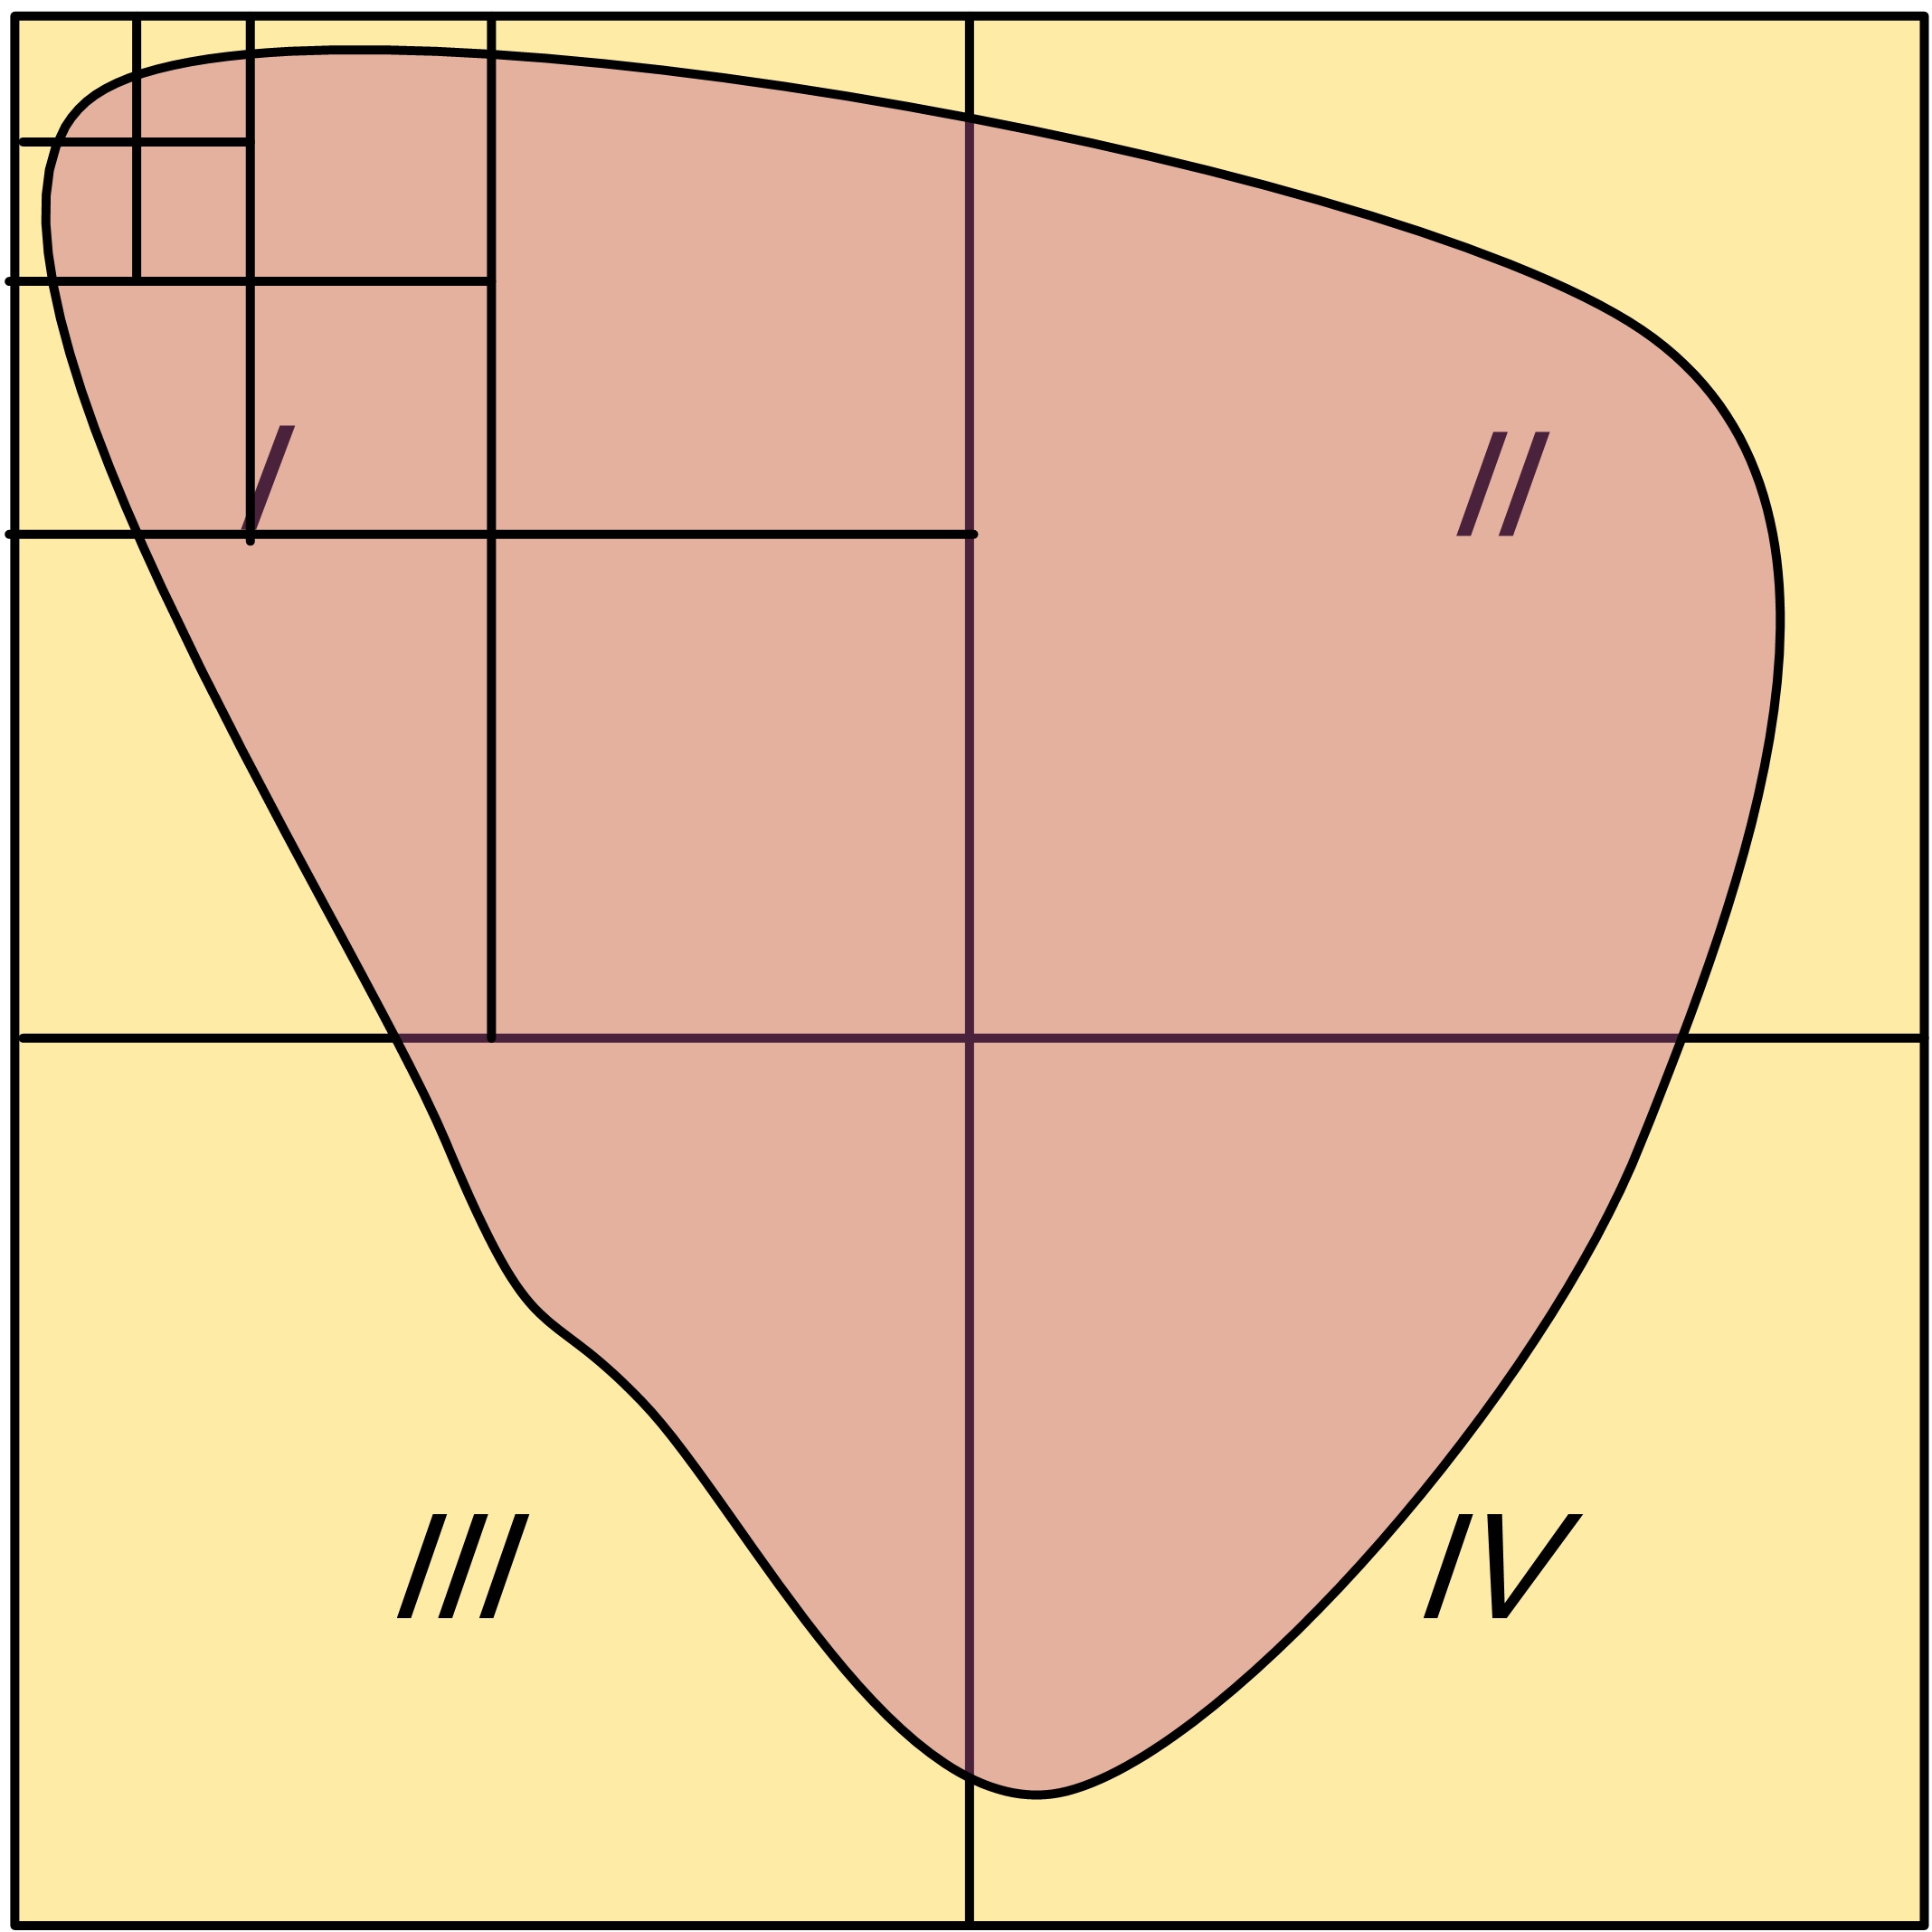
\includegraphics[width=0.3\linewidth]{../../../Untitled}
			\caption{}
			\label{fig:untitled}
		\end{figure}
		
		待定$c>0$,我们对$i=1,2,\cdots,n-1$,如果有$m_{i}\le m_{i+1}$,对于$x\in [x_{i},x_{i}+c]$,我们取
		\begin{equation*}
			q\left( x \right) =\frac{x_i+c-x}{c}m_i+\frac{x-x_i}{c}m_{i+1}
		\end{equation*}
		
		如果有$m_{i}\ge m_{i+1}$,对于$x\in [x_{i}-c,x_{i}]$,我们取
		\begin{equation*}
		q\left( x \right) =\frac{x_i-x}{c}m_i+\frac{x-x_i+c}{c}m_{i+1}
		\end{equation*}
		
		在其它地方令$q(x)=q_{0}(x)$,则$q\in C[a,b],q\le q_{0}\le f$
		
		此时
		\begin{equation*}
			\begin{split}
				\int\limits_a^b{q_0-qdx}=\sum_{i=0}^{n-1}{\int\limits_{x_i}^{x_{i+1}}{q_0-qdx}}=\sum_{i=0}^{n-1}{\int\limits_{x_i}^{x_{i+1}}{\frac{x_i+c-x}{c}m_i+\frac{x-x_i}{c}m_{i+1}-m_i}}dx
				\\
				=\sum_{i=0}^{n-1}{\int\limits_{x_i}^{x_{i+1}}{\frac{x_i-x}{c}m_i+\frac{x-x_i}{c}m_{i+1}}}dx=\sum_{i=0}^{n-1}{\int\limits_{x_i}^{x_{i+1}}{\frac{x_i-x}{c}m_i+\frac{x-x_i}{c}m_{i+1}}}dx
				\\
				=\sum_{i=0}^{n-1}{\frac{\left( m_{i+1}-m_i \right)}{c}\int\limits_{x_i}^{x_{i+1}}{x-x_i}}dx=\sum_{i=0}^{n-1}{\frac{\left( m_{i+1}-m_i \right)}{c}\int\limits_{x_i}^{x_i+c}{x-x_i}}dx=\frac{c}{2}\sum_{i=1}^{n-1}{|m_{i+1}-m_i|}\le \frac{c}{2}\left( n-1 \right) \max \left\{ \mathop {\mathrm{sup}} \limits_{\left[ a,b \right]}f,\mathop {\mathrm{inf}} \limits_{\left[ a,b \right]}f \right\} 
			\end{split}
		\end{equation*}
		
		此时只要$c$充分小,就有
		\begin{equation*}
			\int\limits_a^b{q_0-qdx}\le \frac{\varepsilon}{4}
		\end{equation*}
		
		因此,我们有
		\begin{equation*}
			\int\limits_a^b{f-qdx}=\int\limits_a^b{f-q_0+q_0-qdx}=\int\limits_a^b{f-q_0dx}+\int\limits_a^b{q_0-qdx}\le \frac{\varepsilon}{2}
		\end{equation*}
		
		类似的,我们也可以选取$p\in C[a,b]$,使得
		\begin{equation*}
			f\le p,\int\limits_a^b{f-pdx}\frac{\varepsilon}{2}
		\end{equation*}
		
		此时就有
		\begin{equation*}
			\int\limits_a^b{p-qdx}\le \varepsilon
		\end{equation*}
		
		我们所需要的$p,q$便得出来了
	\end{proof}
	
	我们来点应用
	\begin{exercise}
		$\text{设}\beta _n\rightarrow 0,\text{函数}f\text{在}\left[ -1,2 \right] \text{有界,}\left[ 0,1 \right] \text{黎曼可积,证明}$
		\begin{equation*}
			\lim_{n\rightarrow \infty} \frac{1}{n}\sum_{k=1}^n{f\left( \frac{k}{n}+\beta _n \right)}=\int\limits_0^1{f\left( x \right) dx}
		\end{equation*}
	\end{exercise}
	\begin{proof}
		
		不妨设$f$在$[-1,2]$黎曼可积,只需要说明其在$[0,1]$之外的积分为0即可,即
		\begin{equation*}
			\lim_{n\rightarrow \infty} \frac{1}{n}|\sum_{1\le k\le -n\beta _n\text{或}n\ge k\ge n\left( 1-\beta _n \right)}^{}{f\left( \frac{k}{n}+\beta _n \right)}|\le \lim_{n\rightarrow \infty} \frac{\mathop {\mathrm{sup}} \limits_{\left[ -1,2 \right]}f}{n}\left( 2n\beta _n+1145141919810 \right) =0
		\end{equation*}
		
		于是极限的值集中在$[0,1]$
		
		此时不妨将$f$在$[0,1]$外的值修正为$0$,由先前的结论,存在$p,q\in  \mathbb{R}[x]$,使得
		\begin{equation*}
			p\le f\le q,\int\limits_0^1{qdx}-\varepsilon \le \int\limits_0^1{fdx}\le \int\limits_0^1{pdx}+\varepsilon 
		\end{equation*}
		
		此时
		\begin{equation*}
			\begin{split}
			\lim_{n\rightarrow \infty} \frac{1}{n}\sum_{k=1}^n{f\left( \frac{k}{n}+\beta _n \right)}\le \lim_{n\rightarrow \infty} \frac{1}{n}\sum_{k=1}^n{q\left( \frac{k}{n}+\beta _n \right)}=\int\limits_0^1{q}dx\le \int\limits_0^1{f}dx+\varepsilon 
			\\
			\lim_{n\rightarrow \infty} \frac{1}{n}\sum_{k=1}^n{f\left( \frac{k}{n}+\beta _n \right)}\ge \lim_{n\rightarrow \infty} \frac{1}{n}\sum_{k=1}^n{p\left( \frac{k}{n}+\beta _n \right)}=\int\limits_0^1{p}dx\ge \int\limits_0^1{f}dx-\varepsilon 
			\end{split}
		\end{equation*}
		
		于是乎即可得证
	\end{proof}
	
	\begin{exercise}
		$\text{设}p\ge 1,\int_{\mathbb{R}}{|f\left( x \right) |^pdx}<\infty ,\text{证明}$
		\begin{equation*}
			\lim_{h\rightarrow 0^+} \int_{\mathbb{R}}{|f\left( x+h \right) -f\left( x \right) |^pdx}=0
		\end{equation*}
	\end{exercise}
	\begin{proof}		
		对于$f\in C_{c}(\mathbb{R})$,即$f\in C\left( \mathbb{R} \right) \text{且}cl\left\{ x\in \mathbb{R} :f\left( x \right) =0 \right\} \text{是}\mathbb{R} \text{中紧集,则此时}f\text{是一致连续的}
		$
		
		不妨设$\left[ a,b \right] \supset cl\left\{ x\in \mathbb{R} :f\left( x \right) =0 \right\} $,此时对$h\in(0,1)$,我们有
		\begin{equation*}
			\int_{\mathbb{R}}{|f\left( x+h \right) -f\left( x \right) |^pdx}=\int_{\left[ a,b \right]}{|f\left( x+h \right) -f\left( x \right) |^pdx}
		\end{equation*}
		
		由一致连续性,显然我们有
		\begin{equation*}
			\lim_{h\rightarrow 0^+} \int_{[a,b]}{|f\left( x+h \right) -f\left( x \right) |^pdx}=0
		\end{equation*}
		
		如果我们证明了(证明放在磨光那一部分写),对于一般的满足$\int_{\mathbb{R}}{|f\left( x \right) |^pdx}<\infty$的$f$,如果证明了$\forall \varepsilon >0$存在$g\in C_{c}(\mathbb{R})$,使得
		\begin{equation*}
			\left\| f-g \right\| _{L^p\left( \mathbb{R} \right)}\le \varepsilon 
		\end{equation*}
		
		那么我们就有
		\begin{equation*}
			\begin{split}
				\lim_{h\rightarrow 0^+} \left\| f\left( x+h \right) -f\left( x \right) \right\| _{L^p\left( \mathbb{R} \right)}\le \lim_{h\rightarrow 0^+} \left\| f\left( x+h \right) -g\left( x+h \right) \right\| _{L^p\left( \mathbb{R} \right)}+\left\| g\left( x+h \right) -g\left( x \right) \right\| _{L^p\left( \mathbb{R} \right)}+\left\| f\left( x \right) -g\left( x \right) \right\| _{L^p\left( \mathbb{R} \right)}
				\\
				=2\left\| f\left( x \right) -g\left( x \right) \right\| _{L^p\left( \mathbb{R} \right)}+\lim_{h\rightarrow 0^+} \left\| g\left( x+h \right) -g\left( x \right) \right\| _{L^p\left( \mathbb{R} \right)}\le 2\varepsilon 
			\end{split}
		\end{equation*}
		
		由$\varepsilon$的任意性可知
		\begin{equation*}
			\lim_{h\rightarrow 0^+} \int_{\mathbb{R}}{|f\left( x+h \right) -f\left( x \right) |^pdx}=0
		\end{equation*}
	\end{proof}
	\begin{exercise}
		$\text{设}p\ge 1,\int_{\mathbb{R}}{|f\left( x \right) |^pdx}<\infty ,\text{证明}$
		\begin{equation*}
			\lim_{|h|\rightarrow +\infty} \int_{\mathbb{R}}{|f\left( x-h \right) +f\left( x \right) |^pdx}=2\int_{\mathbb{R}}{|f\left( x \right) |^pdx}
		\end{equation*}
	\end{exercise}
	\begin{proof}
		
		不失一般性,我们考虑在$h\rightarrow +\infty$时候的情况
		
		当$f\in C_{c}(\mathbb{R})$,设$n\in \mathbb{N}$,使得
		\begin{equation*}
			suppf\subset (-n,n)
		\end{equation*}
		
		当$h>2n$时,我们有
		\begin{equation*}
			\begin{split}
				\int_{\mathbb{R}}{|f\left( x \right) +f\left( x-h \right) |^pdx}=\int_{|x|>n}{|f\left( x \right) +f\left( x-h \right) |^pdx}+\int\limits_{-n}^n{|f\left( x \right) +f\left( x-h \right) |^pdx}
				\\
				=\int_{|x|>n}{|f\left( x-h \right) |^pdx}+\int\limits_{-n}^n{|f\left( x \right) |^pdx}
				\\
				=\int_{|x+h|>n}{|f\left( x \right) |^pdx}+\int\limits_{-n}^n{|f\left( x \right) |^pdx}
				\\
				=2\int\limits_{-n}^n{|f\left( x \right) |^pdx}=2\int_{\mathbb{R}}{|f\left( x \right) |^pdx}
			\end{split}
		\end{equation*}
		
		对于一般的满足$\int_{\mathbb{R}}{|f\left( x \right) |^pdx}<\infty$的$f$,如下定义范数
		\begin{equation*}
			\left\| f \right\| _p\triangleq \left( \int\limits_a^b{|f\left( x \right) |^p} \right) ^{\frac{1}{p}}
		\end{equation*}
		
		对任何$\varepsilon >0$,存在$g\in C_{C}^{\infty}\left( \mathbb{R} \right) $,使得
		\begin{equation*}
			\left\| f-g \right\| _p<\frac{\varepsilon}{2+2^{\frac{1}{p}}}
		\end{equation*}
		
		那么此时当$h$充分大,我们有
		\begin{equation*}
			\begin{split}
				|\left\| f\left( x-h \right) +f\left( x \right) \right\| _p-2^{\frac{1}{p}}\left\| f \right\| _p|\le |\left\| f\left( x-h \right) +f\left( x \right) \right\| _p-\left\| g\left( x-h \right) +g\left( x \right) \right\| _p|+|\left\| g\left( x-h \right) +g\left( x \right) \right\| _p-2^{\frac{1}{p}}\left\| g \right\| _p+2^{\frac{1}{p}}\left\| f \right\| _p-\left\| g \right\| _p|
				\\
				\le \left\| f\left( x \right) -g\left( x \right) +f\left( x-h \right) -g\left( x-h \right) \right\| _p+2^{\frac{1}{p}}\left\| f-g \right\| _p\le \left\| f\left( x \right) -g\left( x \right) \right\| _p+\left\| f\left( x-h \right) -g\left( x-h \right) \right\| _p+2^{\frac{1}{p}}\left\| f-g \right\| _p
				\\
				\le \left( 2^{\frac{1}{p}}+2 \right) \left\| f-g \right\| _p=\varepsilon
			\end{split}
		\end{equation*}
	\end{proof}
	

	
	接下来我们来到一个重要的技巧,即函数的磨光,这也是一种逼近技术,只不过是用光滑的(任意阶连续可导)函数逼近一般的函数,并且一般来说,这个光滑函数是一致收敛到我们的目标函数的!而且它保留了原来的函数的各种基本信息,比如单调性,凹凸性这种,同时积分误差(因为一致收敛)将会任意小,所以这是一个很强有力的工具。
	
	它最大的功效就是:原先一个函数,你希望用分部积分,求导,甚至求二阶导这些方式来研究它(或解决问题),但是条件不够,没有光滑性使得这些操作“不合法”,但是假如我允许你如上操作,问题又会变得异常简单,那怎么办?你是否忍不住要导或者积?这样磨光技术就派上用场了,它能使得你的一切操作合理。
	
	\begin{definition}[磨光函数]
		定义$\chi \left( x \right) =\begin{cases}
			\frac{1}{\int\limits_{-1}^1{e^{\frac{1}{1-|x|^2}}dx}}e^{\frac{1}{1-|x|^2}},|x|<1\\
			0,|x|\ge 1\\
		\end{cases}\text{为磨光函数}$,并且$\chi _{\delta}\left( x \right) =\frac{\chi \left( \frac{x}{\delta} \right)}{\delta}\text{,}\delta >0$
		
		其满足:$\chi \in C_{c}^{\infty}\left( \mathbb{R} \right) ,\chi \text{是非负偶函数,}\int_{\mathbb{R}}{\chi}dx=1$
	\end{definition}
	\begin{remark}
		若$f(x)$在$\mathbb{R}$内闭可积,则$f_{\delta}\left( x \right) \triangleq \int\limits_{\mathbb{R}}{f\left( y \right) \chi _{\delta}\left( x-y \right) dy}\in C_{}^{\infty}\left( \mathbb{R} \right) 
		$
	\end{remark}
	
	我们来到一个历史遗留问题
	\begin{example}
		对于一般的满足$\int_{\mathbb{R}}{|f\left( x \right) |^pdx}<\infty$的$f$,如果证明了$\forall \varepsilon >0$存在$g\in C_{c}(\mathbb{R})$,使得
		\begin{equation*}
			\left\| f-g \right\| _{L^p\left( \mathbb{R} \right)}\le \varepsilon 
		\end{equation*}
	\end{example}
	\begin{solution}
		
		这里我们给出两种证明方法
		
		方法一(截断法):
		
		对于$\varepsilon \in (0,1)$,对$f$用之前的结果,我们存在$g \in C(\mathbb{R})$使得
		\begin{equation*}
			\left\| f-g \right\| _{L^p\left( \mathbb{R} \right)}\le  \frac{\varepsilon}{4}
		\end{equation*}
		
		我们取$\delta >0$,使得
		\begin{equation*}
			\int\limits_a^{a+\delta}{|f\left( x \right) |^{p}dx}\le \frac{\varepsilon}{4},\int\limits_{b-\delta}^b{|f\left( x \right) |^{p}dx}\le \frac{\varepsilon}{4},\int\limits_{a+\delta}^{a+2\delta}{|g\left( x \right) |^{p}dx}\le \frac{\varepsilon}{16},\int\limits_{b-2\delta}^{b-\delta}{|g\left( x \right) |^{p}dx}\le \frac{\varepsilon}{16},
		\end{equation*}
		
		设$g_1\left( x \right) =h\left( x \right) g\left( x \right) \in C_c\left( \mathbb{R} \right) ,\text{其中}h\in C^{\infty}\left( \mathbb{R} \right) ,0\le h\left( x \right) \le 1
		$
		
		其中
		
		$h(x)=0,x\in (-\infty,a+\delta)\cup (b-\delta,+\infty)$
		
		$h(x)=1,x\in [a+2\delta,b-2\delta]$
		
		则
		
				$\int\limits_{-\infty}^{+\infty}{|f\left( x \right) -g_1\left( x \right) |^pdx}=\int\limits_a^b{|f\left( x \right) -h\left( x \right) g\left( x \right) |^pdx}=\int\limits_a^{a+\delta}{|f\left( x \right) -h\left( x \right) g\left( x \right) |^pdx}+\int\limits_{a+\delta}^{b-\delta}{|f\left( x \right) -h\left( x \right) g\left( x \right) |^pdx}+\int\limits_{b-\delta}^b{|f\left( x \right) -h\left( x \right) g\left( x \right) |^pdx}$
				
				$=\int\limits_a^{a+\delta}{|f\left( x \right) |^pdx}+\int\limits_{b-\delta}^b{|f\left( x \right) |^pdx}+\int\limits_{a+\delta}^{b-\delta}{|f\left( x \right) -h\left( x \right) g\left( x \right) |^pdx}=\int\limits_a^{a+\delta}{|f\left( x \right) |^pdx}+\int\limits_{b-\delta}^b{|f\left( x \right) |^pdx}+\int\limits_{a+\delta}^{b-\delta}{|f\left( x \right) -g\left( x \right) +g\left( x \right) -h\left( x \right) g\left( x \right) |^pdx}$
				
				$\le \int\limits_a^{a+\delta}{|f\left( x \right) |^pdx}+\int\limits_{b-\delta}^b{|f\left( x \right) |^pdx}+\int\limits_{a+\delta}^{b-\delta}{|f\left( x \right) -g\left( x \right) |^pdx}+\int\limits_{a+\delta}^{b-\delta}{|g\left( x \right) -h\left( x \right) g\left( x \right) |^pdx}$
				
				$\le \int\limits_a^{a+\delta}{|f\left( x \right) |^pdx}+\int\limits_{b-\delta}^b{|f\left( x \right) |^pdx}+\int\limits_a^b{|f\left( x \right) -g\left( x \right) |^pdx}+\int\limits_{a+\delta}^{b-\delta}{|g\left( x \right) -h\left( x \right) g\left( x \right) |^pdx}$
				
				$\le \int\limits_a^{a+\delta}{|f\left( x \right) |^pdx}+\int\limits_{b-\delta}^b{|f\left( x \right) |^pdx}+\int\limits_a^b{|f\left( x \right) -g\left( x \right) |^pdx}+\int\limits_{a+\delta}^{a+2\delta}{|g\left( x \right) -h\left( x \right) g\left( x \right) |^pdx}+\int\limits_{a+2\delta}^{b-2\delta}{|g\left( x \right) -h\left( x \right) g\left( x \right) |^pdx}+\int\limits_{b-2\delta}^{b-\delta}{|g\left( x \right) -h\left( x \right) g\left( x \right) |^pdx}$
				
				$\le \frac{3\varepsilon}{4}+\int\limits_{a+\delta}^{a+2\delta}{|g\left( x \right) -h\left( x \right) g\left( x \right) |^pdx}+\int\limits_{b-2\delta}^{b-\delta}{|g\left( x \right) -h\left( x \right) g\left( x \right) |^pdx}$
				
				$\le \frac{3\varepsilon}{4}+\int\limits_{a+\delta}^{a+2\delta}{|g\left( x \right) |^pdx}+\int\limits_{b-2\delta}^{b-\delta}{|g\left( x \right) |^pdx}=\varepsilon $
				
				这样就很套路地解决了这道题,截断法的思路大多是连续逼近,然后手动截断。
				
		方法二(磨光法)
		
		第一步,紧支化:
		\begin{equation*}
			\forall \varepsilon>0,\text{取}n\in \mathbb{N},\text{使得}2^p\int_{|x|>n}{|f\left( x \right) |^pdx}\le \varepsilon
		\end{equation*}
		
		我们取$h\in C_{c}^{\infty}\left( \mathbb{R} \right)$,使得$h(x)=1,x\in (-n,n),0\le h(x)\le 1,\forall x\in \mathbb{R}$
		
		即
		\begin{equation*}
			\int_{\mathbb{R}}{|h\left( x \right) f\left( x \right) -f\left( x \right) |dx=}\int_{|x|>n}{|h\left( x \right) f\left( x \right) -f\left( x \right) |dx\le}2^p\int_{|x|>n}{|f\left( x \right) |^pdx}\le \varepsilon 
		\end{equation*}
		
		此时我们证明了$f$有紧支撑
		
		第二步,磨光
		
		我们引用磨光核$ \chi \in C_{c}^{\infty}\left( \mathbb{R} \right) ,\text{使得}$
		\begin{equation*}
			\int_{\mathbb{R}}{\chi \left( x \right) dx}=1
		\end{equation*}
		($\chi$为非负偶函数且$0\le\chi\le1$)
		
		令$\chi _{\varepsilon}=\frac{1}{\varepsilon}\chi \left( \frac{x}{\varepsilon} \right) ,\text{我们考虑卷积}f*\chi _{\varepsilon}\in C_{c}^{\infty}\left( \mathbb{R} \right) ,\text{运用卷积不等式,我们有}
		$
		\begin{equation*}
			\left\| f*\chi _{\varepsilon} \right\| _{L^p}\le C\left\| f \right\| _{L^p},\text{由此我们可以证明}\lim_{\varepsilon \rightarrow 0} \left\| f*\chi _{\varepsilon}-f \right\| _{L^p}=0
		\end{equation*}
		
		于是我们有
		\begin{equation*}
			f_{\delta}\left( x \right) =\int\limits_{\mathbb{R}}{f\left( y \right) \chi _{\delta}\left( x-y \right) dy}\overset{y=x-\delta y}{=}\int\limits_{\mathbb{R}}{f\left( x-\delta y \right) \chi \left( y \right) dy}=\int\limits_{-1}^1{f\left( x-\delta y \right) \chi \left( y \right) dy}	
		\end{equation*}
		
		当$x\notin[-n-\delta,n+\delta]$,则$x-\delta y \notin[-n,n]$
		
		因此$f_{\delta}\left( x \right) =0,x\notin[-n-\delta,n+\delta],\forall y\in[-1,1]$
		
		直观上,$f_{\delta}$的支撑比原来的大了$\delta$的距离
		
		于是$f_{\delta}\in C_{c}^{\infty}\left( \mathbb{R} \right) $
		
		我们有
		\begin{equation*}
			\left\| f_{\delta}-f \right\| _p=\left\| \int\limits_{\mathbb{R}}{f\left( x-\delta y \right) \chi \left( y \right) dy}-\int\limits_{\mathbb{R}}{f\left( x \right) \chi \left( y \right) dy} \right\| _p=\left\| \int\limits_{\mathbb{R}}{\left( f\left( x-\delta y \right) -f\left( x \right) \right) \chi \left( y \right) dy} \right\| _p\le \int\limits_{-1}^1{\left\| \left( f\left( x-\delta y \right) -f\left( x \right) \right) \right\| _p\chi \left( y \right) dy}
		\end{equation*}
		
		由勒贝格积分的连续性,我们有
		\begin{equation*}
			\lim_{h\rightarrow 0} \left\| \left( f\left( x-h \right) -f\left( x \right) \right) \right\| _p=0
		\end{equation*}
		
		注意到$\forall y\in[-1,1],\delta y$一致趋向于0,则
		\begin{equation*}
			\lim_{\delta \rightarrow 0} \left\| f_{\delta}-f \right\| _p\le \lim_{\delta \rightarrow 0} \int\limits_{-1}^1{\left\| \left( f\left( x-\delta y \right) -f\left( x \right) \right) \right\| _p\chi \left( y \right) dy}=0
		\end{equation*}
		
		于是我们得证
	\end{solution}
	
	\begin{example}
		$f\in C^{1}(\mathbb{R})$,且$|f\left( x+t \right) -2f\left( x \right) +f\left( x-t \right) |\le Mt^2$
		,证明
		\begin{equation*}
			|f'(x+t)-f'(x)|\le M|t|
		\end{equation*}
	\end{example}
	\begin{proof}
		若$f$光滑,则
		\begin{equation*}
			\begin{aligned} 
				\underset{t\rightarrow 0^+}{\lim}\frac{|f\left( x+t \right) -2f\left( x \right) +f\left( x-t \right) |}{t^2}
				 &=\underset{t\rightarrow 0^+}{\lim}\frac{|f'\left( x+t \right) -f'\left( x-t \right) |}{2t}\\	
				&=\underset{t\rightarrow 0^+}{\lim}\frac{|f''\left( x+t \right) +f''\left( x-t \right) |}{2}\\
				&= \left| f''(x)\right| \le M,\forall x \in \mathbb{R}
			\end{aligned}
		\end{equation*}
		
		由拉格朗日中值定理,可得
		\begin{equation*}
			|f'(x+t)-f'(x)|=|t|\left| f''(x)\right|\le M|t|
		\end{equation*}
		
		这样就结束了,但事实上$f$不一定光滑,我们考虑将其磨光
		
		即
			\begin{equation*}
			f_{\delta}\left( x \right) =\int\limits_{\mathbb{R}}{f\left( y \right) \chi _{\delta}\left( x-y \right) dy}\overset{y=x-\delta y}{=}\int\limits_{\mathbb{R}}{f\left( x-\delta y \right) \chi \left( y \right) dy}	
		\end{equation*}
		
		于是乎
		\begin{equation*}
			|f_{\delta}\left( x+t \right) -2f_{\delta}\left( x \right) +f_{\delta}\left( x-t \right) \le \int_{\mathbb{R}}{|f\left( x+t-\delta y \right)}-2f\left( x-\delta y \right) +f\left( x-t-\delta y \right) |\chi \left( y \right) dy\le M|t|^2\int_{\mathbb{R}}{\chi \left( y \right) dy}=M|t|^2
		\end{equation*}
		
	现在我们就有
	\begin{equation*}
		|f'_{\delta}(x+t)-f'_{\delta}(x)|\le M|t|
	\end{equation*}
	
	又因为
	\begin{equation*}
		f\prime_{\delta}\left( x \right) =\frac{1}{\delta}\int_{\mathbb{R}}{f\left( y \right) \chi _{\delta}\prime\left( x-y \right) dy}=-\int_{\mathbb{R}}{f\left( y \right) d\chi _{\delta}\left( x-y \right)}\overset{\text{分部积分}}{=}\mathop {-f\left( y \right) \chi _{\delta}\left( x-y \right)} \limits_{=0}+\int_{\mathbb{R}}{f\prime\left( y \right) \chi _{\delta}\left( x-y \right)}dy
	\end{equation*}
	
	于是我们有
	\begin{equation*}
		|f\prime_{\delta}\left( x \right) -f\prime\left( x \right) |=|\int_{\mathbb{R}}{\left( f\prime\left( x-\delta y \right) -f\prime\left( x \right) \right) \chi _{\delta}\left( y \right)}dy|\le \int_{|y|\le 1}{|\left( f\prime\left( x-\delta y \right) -f\prime\left( x \right) \right) |\chi _{\delta}\left( y \right)}dy
	\end{equation*}
	
	由于$f'$连续,$\delta y$关于$
	y\in [-1,1]$一致趋向于0.于是
	\begin{equation*}
		\lim_{\delta \rightarrow 0^+} |f\prime_{\delta}\left( x \right) -f\prime\left( x \right) |\le \lim_{\delta \rightarrow 0^+} \int_{\mathbb{R}}{|\left( f\prime\left( x-\delta y \right) -f\prime\left( x \right) \right) |\chi _{\delta}\left( y \right)}dy=0
	\end{equation*}
	则结论得证
	\end{proof}
	
	接下来我们来证明一下非连续版本的黎曼定理\begin{example}
		$\text{设}A\subset \mathbb{R} \text{是集合,}f\text{在}A\text{上绝对可积},g\text{是周期}T>0\text{的有界可积函数}$,则
		\begin{equation*}
			\lim_{x\rightarrow +\infty} \int_A{f\left( y \right) g\left( xy \right)}dy=\frac{1}{T}\int_A{f\left( y \right) dy}\int\limits_0^T{g\left( y \right) dy}
		\end{equation*}
	\end{example}
	\begin{proof}
		
		我们不妨假设$A=\mathbb{R}$,否则在$A$外补充$f$定义为0
		
		现考虑磨光函数$f_{\delta},g_{\delta}\in C^{\infty}(\mathbb{R})$
		
		此时对$f_{\delta}$我们有
		\begin{equation*}
			|f_{\delta}\left( x \right) |=|\int_{\mathbb{R}}{f\left( x \right) \chi _{\delta}\left( x-y \right) dy}|\le \int_{\mathbb{R}}{|f\left( x \right) |\chi _{\delta}\left( x-y \right) dy}\le \frac{\mathrm{sup}\chi}{\delta}\int_{\mathbb{R}}{|f\left( x \right) |dy}
		\end{equation*}
		
		此时对$g_{\delta}$我们有
		\begin{equation*}
			g_{\delta}\left( x+T \right) =\int_{\mathbb{R}}{g\left( x+T \right) \chi _{\delta}\left( x-y \right) dy}=g_{\delta}\left( x \right)
		\end{equation*}
		
		于是由连续版本的黎曼定理,结论显然成立(具体证明过程需要大家掌握)
		
		现在就有
		\begin{equation*}
			\lim_{x\rightarrow +\infty} \int_A{f_{\delta}\left( y \right) g_{\delta}\left( xy \right)}dy=\frac{1}{T}\int_A{f_{\delta}\left( y \right) dy}\int\limits_0^T{g_{\delta}\left( y \right) dy}
		\end{equation*}
		
		于是
		
		$|\int_A{f\left( y \right) g\left( xy \right)}dy-\frac{1}{T}\int_A{f\left( y \right) dy}\int\limits_0^T{g\left( y \right) dy}|
		\\
		=|\int_A{f\left( y \right) g\left( xy \right)}dy-\int_A{f_{\delta}\left( y \right) g_{\delta}\left( xy \right)}dy+\int_A{f_{\delta}\left( y \right) g_{\delta}\left( xy \right)}dy-\frac{1}{T}\int_A{f_{\delta}\left( y \right) dy}\int\limits_0^T{g_{\delta}\left( y \right) dy}+\frac{1}{T}\int_A{f_{\delta}\left( y \right) dy}\int\limits_0^T{g_{\delta}\left( y \right) dy}-\frac{1}{T}\int_A{f\left( y \right) dy}\int\limits_0^T{g\left( y \right) dy}|
		\\
		\le |\int_A{f\left( y \right) g\left( xy \right)}dy-\int_A{f_{\delta}\left( y \right) g_{\delta}\left( xy \right)}dy|+|\int_A{f_{\delta}\left( y \right) g_{\delta}\left( xy \right)}dy-\frac{1}{T}\int_A{f_{\delta}\left( y \right) dy}\int\limits_0^T{g_{\delta}\left( y \right) dy}|+|\frac{1}{T}\int_A{f_{\delta}\left( y \right) dy}\int\limits_0^T{g_{\delta}\left( y \right) dy}-\frac{1}{T}\int_A{f\left( y \right) dy}\int\limits_0^T{g\left( y \right) dy}|
		$
		
		注意到		
		\begin{equation*}
			\begin{aligned}
				|\int_A{f\left( y \right) g\left( xy \right)}dy-\int_A{f_{\delta}\left( y \right) g_{\delta}\left( xy \right)}dy|&=|\int_A{f\left( y \right) g\left( xy \right)}dy-\int_A{f_{\delta}\left( y \right) g\left( xy \right)}dy+\int_A{f\left( y \right) g_{\delta}\left( xy \right)}dy-\int_A{f_{\delta}\left( y \right) g_{\delta}\left( xy \right)}dy|
				\\
				&\le |\int_A{f\left( y \right) g\left( xy \right)}dy-\int_A{f_{\delta}\left( y \right) g\left( xy \right)}dy|+|\int_A{f_{\delta}\left( y \right) g\left( xy \right)}dy-\int_A{f_{\delta}\left( y \right) g_{\delta}\left( xy \right)}dy|
				\\
				&=|\int_A{\left[ f\left( y \right) -f_{\delta}\left( y \right) \right] g\left( xy \right) dy}|+|\int_A{f_{\delta}\left( y \right) \left[ g\left( xy \right) -g_{\delta}\left( xy \right) \right]}dy|
				\\
				&\le \mathrm{sup}|g||\int_A{f\left( y \right) -f_{\delta}\left( y \right)}dy|+\frac{\frac{\mathrm{sup}\chi}{\delta}\int_{\mathbb{R}}{|f\left( x \right) |dy}}{x}|\int_A{g\left( xy \right) -g_{\delta}\left( xy \right)}dy|
			\end{aligned}
		\end{equation*}	
	
	此时,我们令$x \rightarrow +\infty$有
	\begin{equation*}
		|\int_A{f\left( y \right) g\left( xy \right)}dy-\frac{1}{T}\int_A{f\left( y \right) dy}\int\limits_0^T{g\left( y \right) dy}|\le \mathrm{sup}|g||\int_A{f\left( y \right) -f_{\delta}\left( y \right)}dy|+|\frac{1}{T}\int_A{f_{\delta}\left( y \right) dy}\int\limits_0^T{g_{\delta}\left( y \right) dy}-\frac{1}{T}\int_A{f\left( y \right) dy}\int\limits_0^T{g\left( y \right) dy}|
	\end{equation*}	
	再令$\delta \rightarrow 0^{+}$,就有
	\begin{equation*}
		\lim_{x\rightarrow +\infty}|\int_A{f\left( y \right) g\left( xy \right)}dy-\frac{1}{T}\int_A{f\left( y \right) dy}\int\limits_0^T{g\left( y \right) dy}|=0
	\end{equation*}
	
	得证
	\end{proof}		
\end{document}